\chapter{Configurable Timed CEGAR} \label{chap:timed_cegar}

This chapter presents a configurable framework for CEGAR-based reachability analysis of timed automata. First, the goal of the framework is explained, than the used algorithms and techniques are enumerated and finally, the extensibility of the framework presented. 

\section{Generic CEGAR framework}

The key idea of the framework is to provide various techniques for each phases of the CEGAR-loop, by using correspondent parts of CEGAR-based reachability algorithms. Most of these algorithms already exist (mostly for other formalisms, and they have to be adapted to timed automata), but some of them are new contributions. The created modules can then be combined to form new algorithms (that is, the technique used in each phase of CEGAR can be provided by different algorithms), and choosing the most efficient parts of the original algorithms can result in an even more efficient algorithm than the original ones. 

The architecture of the framework is illustrated in Figures \ref{fig:cegaraut} and \ref{fig:cegarssp}. There are two different realizations of the CEGAR-loop, because the framework supports two distinct ways to apply abstraction to timed automata. While the first approach (Figure \ref{fig:cegaraut}) is based on eliminating clock variables (see Section \ref{sec:cegarex}):  starting from a finite automaton (without any clock variables) the current automaton gets extended with some clocks in each iteration -- and the \emph{automaton} is the base of refinement, the other (Figure \ref{fig:cegarssp}) is based on the refinement of the \emph{state space} itself. Only techniques of the same approach are interchangeable -- hence the two realizations.

\subsection{Automaton-based refinement}

\begin{figure} 
	\centering
	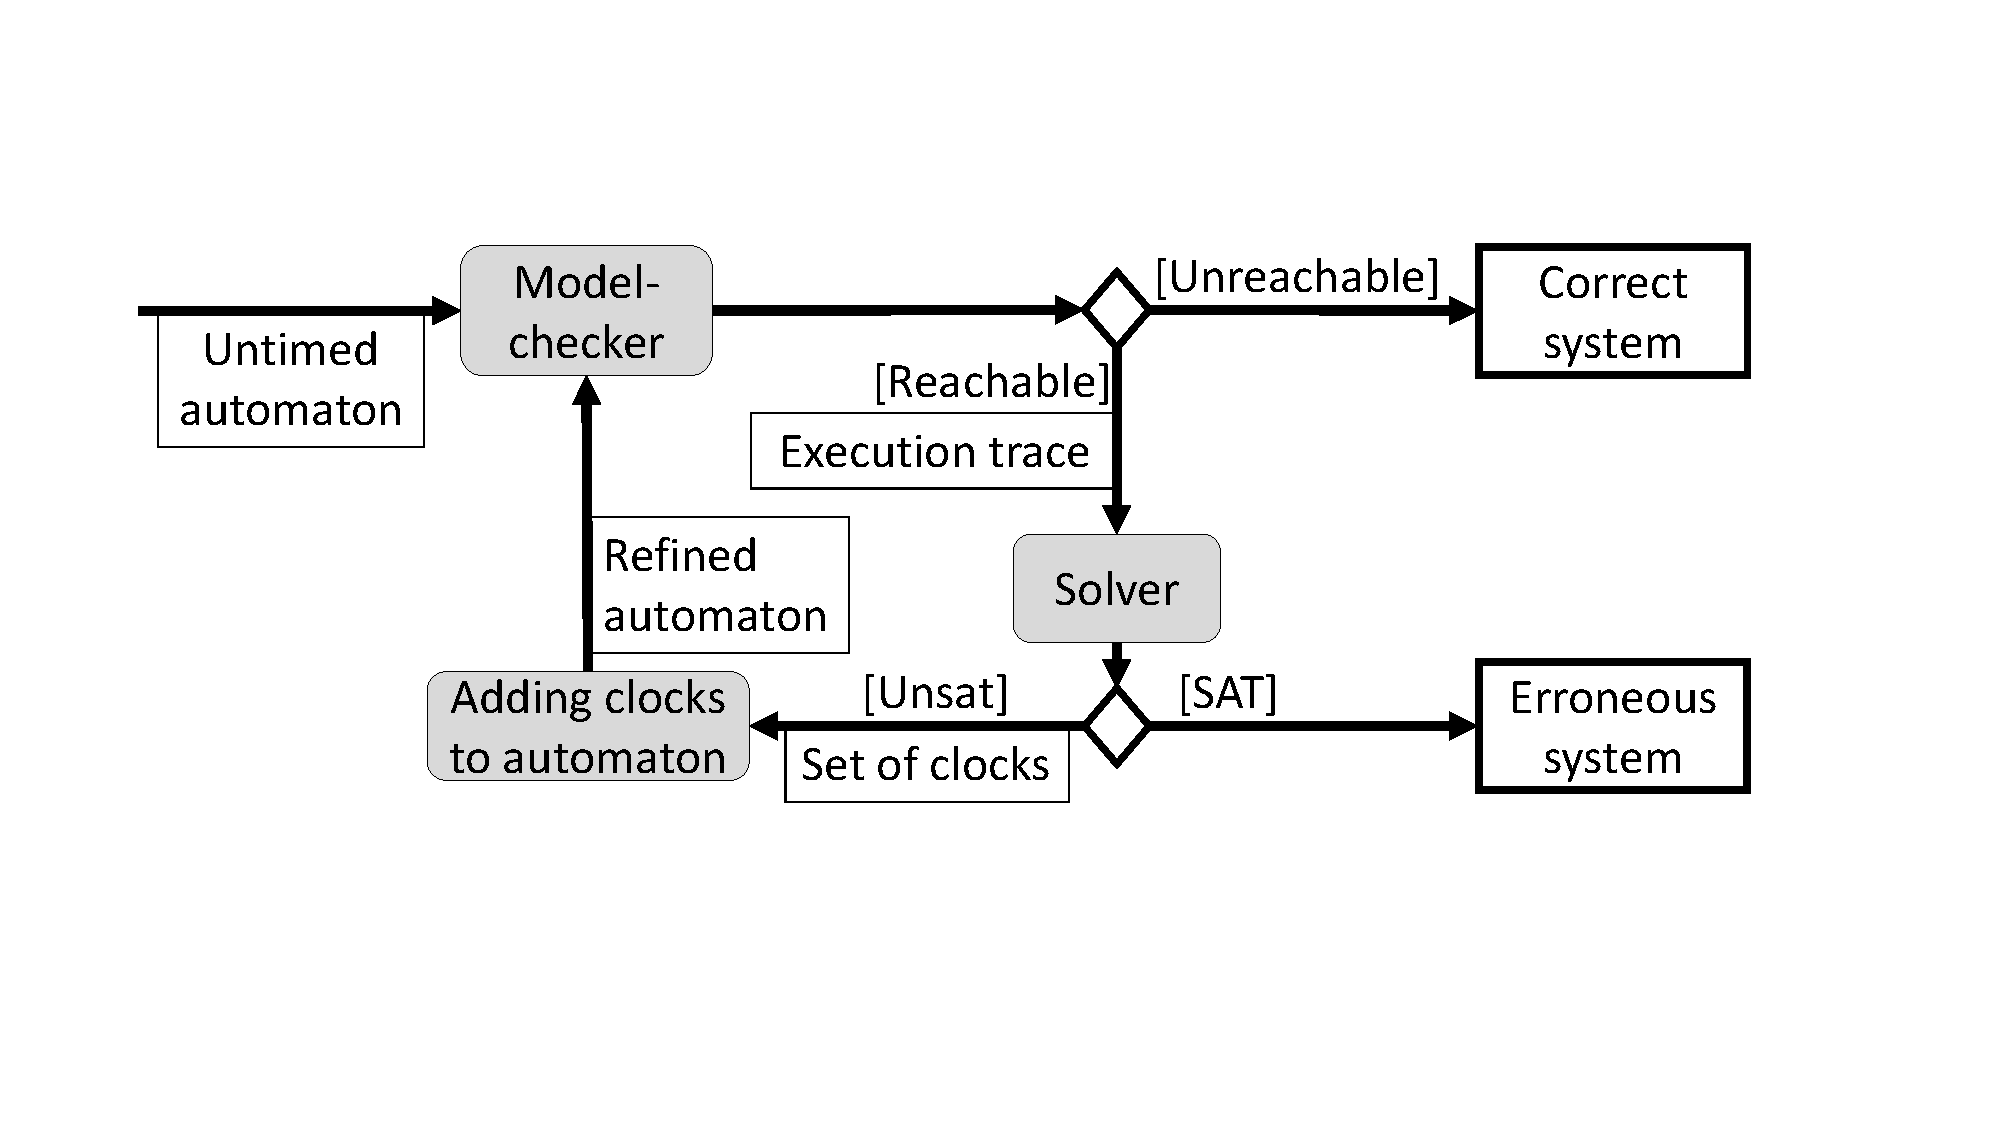
\includegraphics[width=.7\textwidth]{include/figures/alg_arch_ta}%
	\caption{Automaton-based refinement}%
	\label{fig:cegaraut}%
\end{figure}

Figure \ref{fig:cegaraut} depicts the architecture of the automaton-based approach. The initial abstraction is a finite automaton that is derived from the original timed automaton by removing all clock variables and clock constraints. 

In each iteration of the CEGAR-loop, the task of the model checking phase is to determine whether the error location is reachable in the current automaton and provide a trace (counterexample) if there is one. Therefore, this phase should be realized by a reachability-checking algorithm for timed automata that can find a trace to the location.

The task of the analysis phase is to check if the trace found is feasible in the original automaton and if it isn't, provide a set of clock variables that can then be added to the automaton (with the clock constraints they appear in) so that the model checker won't find this counterexample again. This can be calculated by a solver.

Finally, the only task of the refinement phase is to refine the current abstraction of the automaton, by extending it with the given set of clock variables (and the constraints they appear in). The task is straightforward, and so there is only one technique for this phase of the CEGAR-loop (in case of automaton refinement).

\begin{algorithm}
	\KwIn{$\mathcal{A}_\mathcal{C}=\langle L,l_0,E,I \rangle$, $l_{err} \in L$}
	\KwOut{$\sigma=l_0 \xrightarrow{t_0} l_1 \xrightarrow{t_1} \cdots \xrightarrow{t_n} l_{err}$ if $l_{err}$ is reachable, \emph{No} otherwise}
	\BlankLine
	$\mathcal{A} \leftarrow \mathcal{A}_\mathcal{C} \setminus \mathcal{C}$  \tcc*{initial abstraction}
	\While{\emph{true}}{
		$\sigma \leftarrow$ reachable($\mathcal{A},l_{err}$) \tcc*{model checking}
		\eIf(\tcc*[f]{no counterexample is found}){$\not\exists \sigma$}
		{\KwRet{\emph{No}}\tcc*{unreachable}}
		{$C \leftarrow$ refinementset($\mathcal{A},\sigma$)  \tcc*{analysis} 
			\eIf(\tcc*[f]{No refinement set, because feasible}){$c=\emptyset$}{\KwRet{$\sigma$}\;}
			{$\mathcal{A} \leftarrow$ refine($\mathcal{A},C,\mathcal{A}_\mathcal{C}$)\tcc*{automaton is refined by $C$}}
		}
	}
	\caption{Automaton-based refinement} \label{alg:ceraraut}
\end{algorithm}


Algorithm \ref{alg:ceraraut} provides pseudocode for the described approach. Functions \emph{reachable()}, \emph{refinementset()} and \emph{refine()} are components that can be chosen from the techniques described in
the following sections, where two reachability algorithms, an approach for calculating the clocks to include, and the algorithm for refining the automaton are presented. Algorithms are demonstrated on the automaton in Figure \ref{fig:loopinfinite} with $l_{err}=\text{\emph{end}}$ to ease understanding. From now on $\mathcal{A}$ will refer to that particular timed automaton.

\subsubsection{Zone graph exploration} 

\begin{figure} [h]
	\centering
	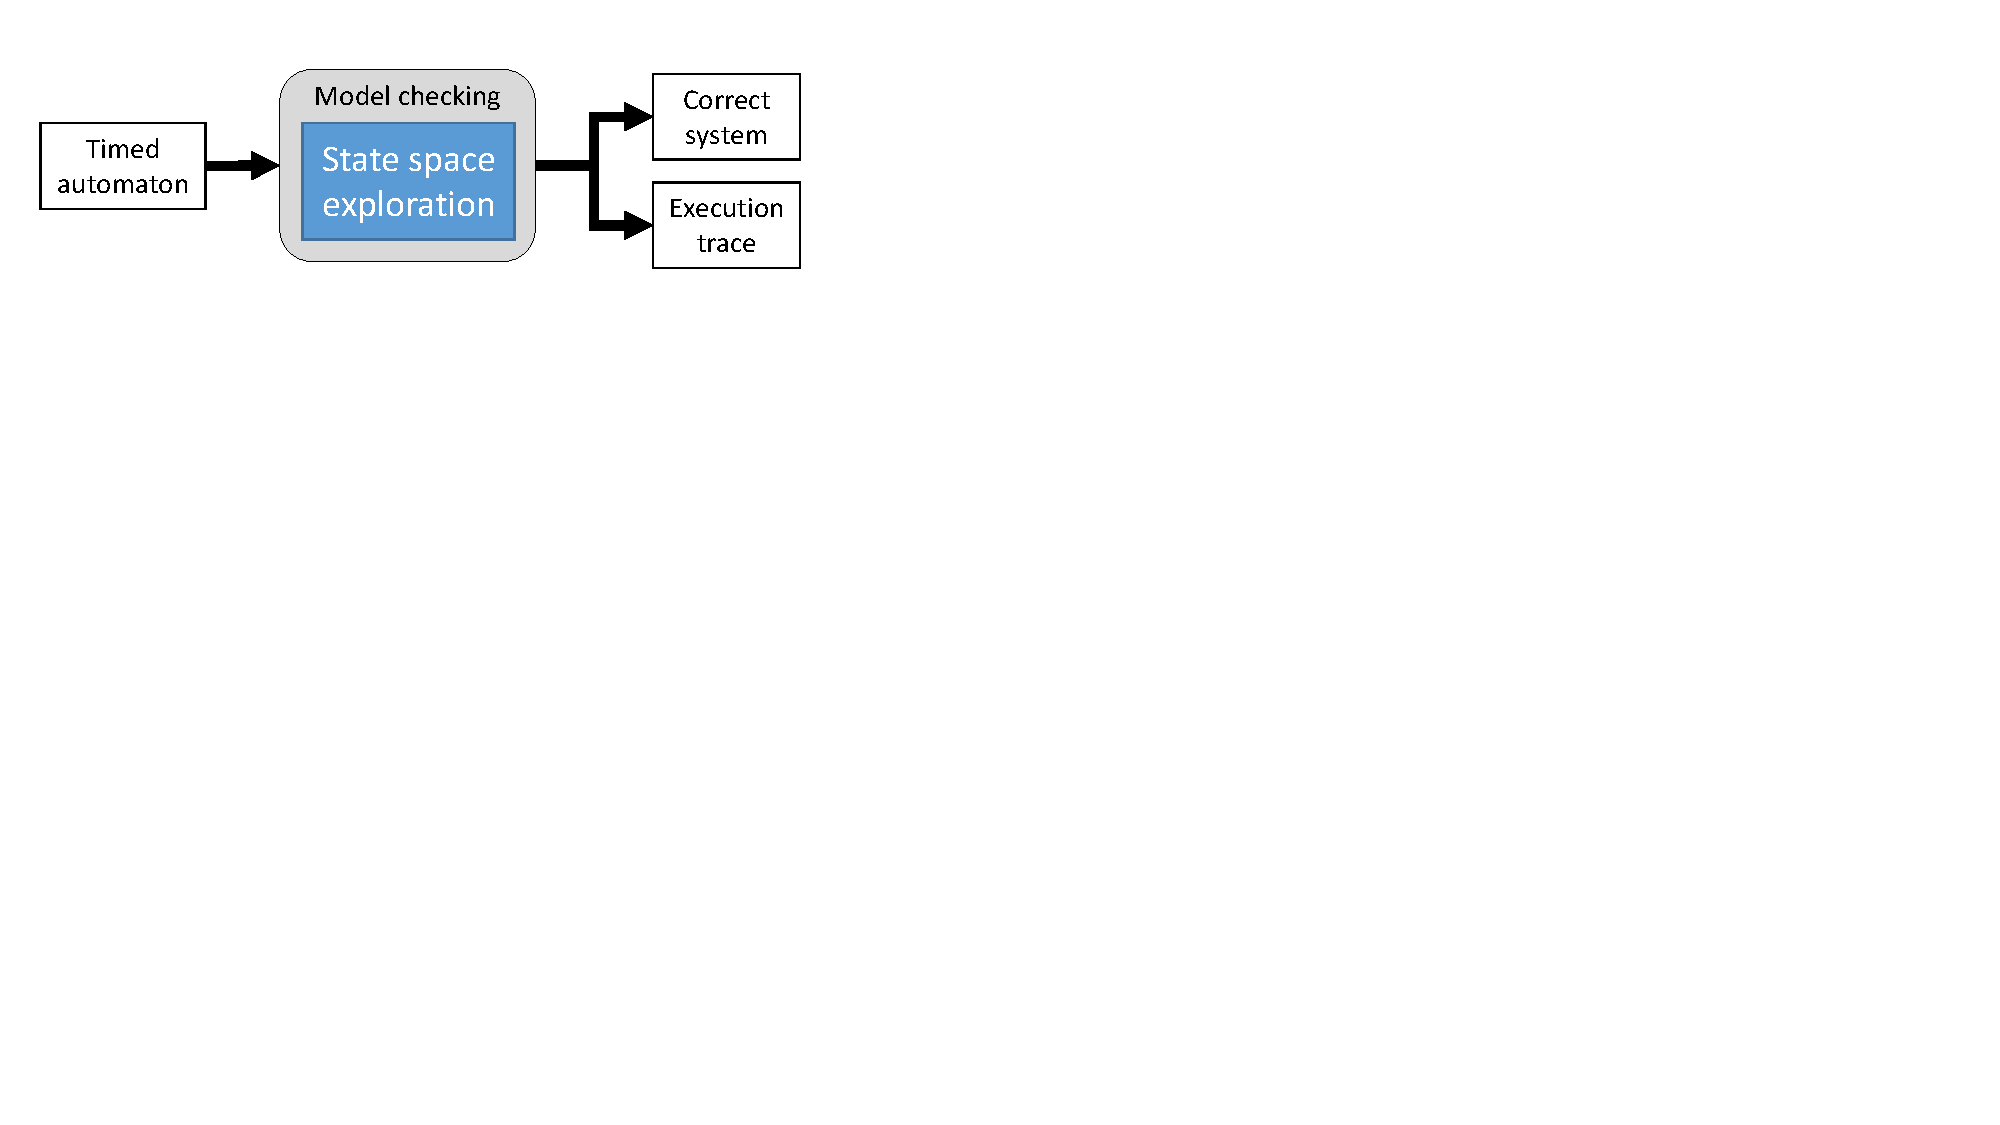
\includegraphics[width=.7\textwidth]{include/figures/modules_ta_mc}
	%\caption{Statespace-based refinement}
	%\label{fig:cegarssp}
\end{figure}

The reachability-checking algorithm described in Section \ref{sec:tareach} is an obvious choice for the model checking phase, however, it is important to note that the algorithm does not handle discerete variables. The discrete valuation can be encoded into the location (and calculated on the fly) but in this case termination is not ensured (as Section \ref{sec:extfa} explains).

\subsubsection{Satisfiability-based model checker}\label{sec:satmc}

\begin{figure}[h]
	\centering
	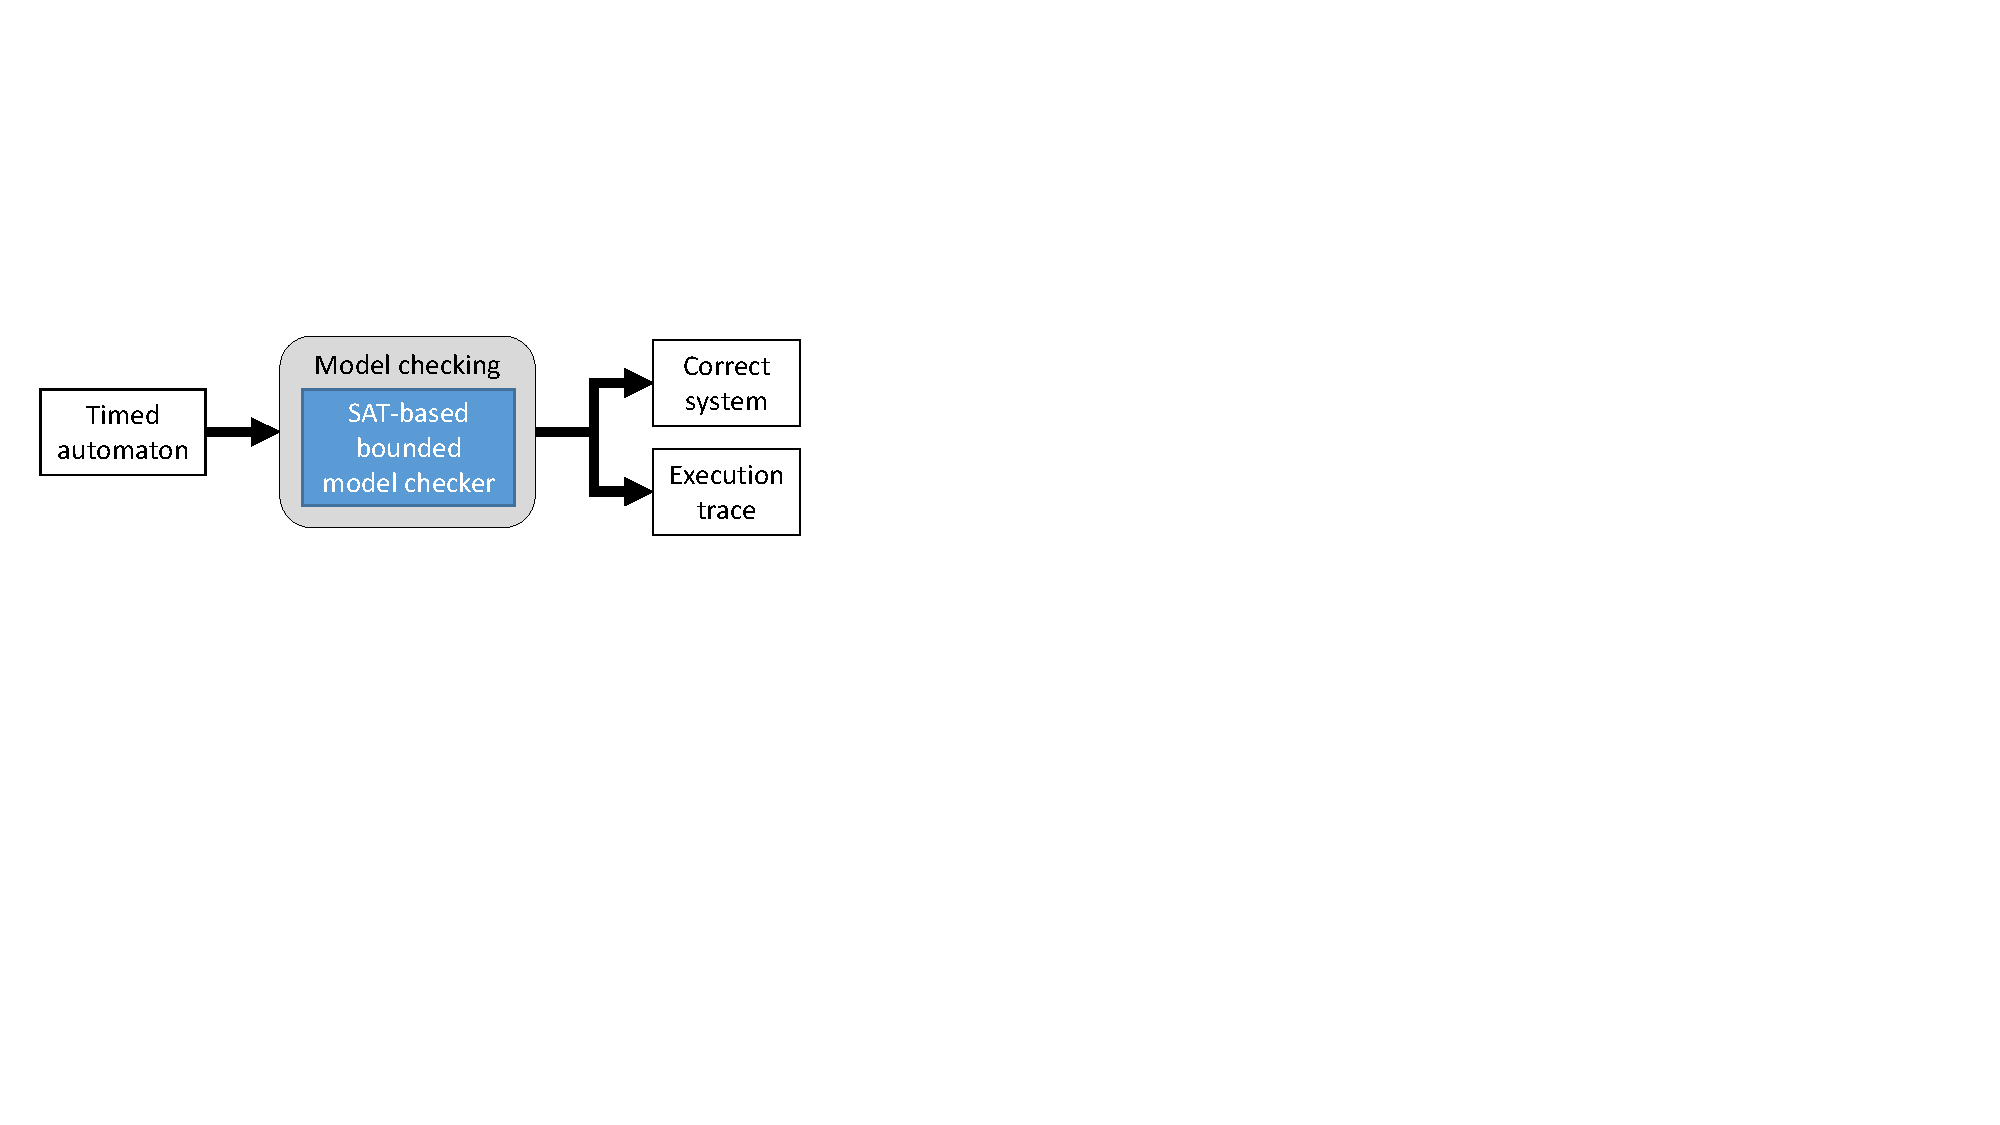
\includegraphics[width=.7\textwidth]{include/figures/modules_ta_mc_sat}
	%\caption{Statespace-based refinement}
	%\label{fig:cegarssp}
\end{figure}

Satisfiability-based model checking as introduced in Section \ref{sec:cegarex} can be directly applied to timed automata -- the only necessary change is to define a transformation that can turn a counterexample (an execution trace) into an SMT-problem.

The idea is to separate discrete transitions from time transitions. Consider a counterexample sequence $\sigma = l_0 \xrightarrow{t_0} l_1 \xrightarrow{t_1} \cdots \xrightarrow{t_n} l_{err}$.  This representation of $\sigma$ hides the fact that it is important how much time the system spends in each location -- i.e. delay transitions. Let us denote the amount of time spent in $l_i$ by $d_i$. This way $\sigma$ can be defined by $\sigma = l_0 \xrightarrow{d_0} \xrightarrow{t_0} l_1 \xrightarrow{d_1} \xrightarrow{t_1} \cdots \xrightarrow{d_n} \xrightarrow{t_n} l_{err}$. In this representation $\xrightarrow{d_i}$ can be considered a special kind of transition that increases $v(c)$ for each $c \in \mathcal{C}$ by $d_i$. Based on this the SMT formula can be constructed.

First, let us assign a variable for each clock in each location, both before and after the delay -- that is, this means $2\cdot n \cdot \abs{\mathcal{C}}$ variables. Let us denote these variables by $c_i$ (for the value of clock $c$ in location $l_i$ before the delay) and $c_i'$ (for the value of clock $c$ in location $l_i$ after the delay). Let us also assign variables for each $d_i$. The first constraints that have to be added is that each of the defined variables are greater or equal to 0.

The initial constraints can simply be described by $c_0 =0$ for each $c \in \mathcal{C}$. Delay transitions can be turned into constraints by the following equation $c_i+d_i=c_i'$ for each $c \in \mathcal{C}, 0 \leq i \leq n$. In case of discrete transitions, guards (clock constraints) can be turned into SMT constraints by replacing the clock variables with the defined variables. The guard $g_i$ of a transition $t_i(l_i,g_i,r_i,l_{i+1})$ can be transformed by replacing all clocks $c$ appearing in $g_i$ by $c_i'$. Resets can also be simply transformed into constraints -- for all $c \in r_i$ $c_{i+1}=0$ has to be added to the set of constraints. Note, that this way $c_{i+1}$ is only specified for the reset clocks. For all $c \not\in r_i$ $c_{i+1}=c_i'$ has to be added to the set of constraints. Invariants can be transformed into SMT constraints the same way as guards.

Discrete variables can be mapped to SMT variables as before since discrete variables and clock variables have no affect on each other.


\begin{runningExample}
	Consider automaton $\mathcal{A}$ (recall, it is the automaton depicted in Figure \ref{fig:loopinfinite}). Assume the counterexample is $\sigma= \text{\emph{start}} \to \text{\emph{loop}} \to \text{\emph{end}}$. The new variables are $x_0$,$y_0$,$x_0'$,$y_0'$,$x_1$,$y_1$,$x_1'$,$y_1'$,$x_2$,$y_2$,$x_2'$,$y_2'$,$d_0$,$d_1$ and $d_2$. It is important to define them to be non-negative since they represent the elapse of time. Initial constraints are $x_0=0$ and $y_0=0$. Delay is described by constraints $x_0'=x_0+d_0$, $y_0'=y_0+d_0$, $x_1'=x_1+d_1$, $y_1'=y_1+d_1$, $x_2'=x_2+d_2$ and $y_2'=y_2+d_2$.
	
	There is no guard on edge \emph{start} $\to$ \emph{loop}, but it resets both variables yielding the constraints $x_1=0$, $y_1=0$. The invariant of location \emph{loop} can be transformed to $x_1 \leq 10$ and $x_1' \leq 10$. The next edge has a guard, $y \geq 20$ that can be transformed to $y_1' \geq 20$, and the resets to $x_2=0$ and $y_2=0$. This results in the formula $\varphi=x_0=0 \wedge y_0=0 \wedge x_0'=x_0+d_0 \wedge y_0'=y_0+d_0 \wedge x_1'=x_1+d_1 \wedge y_1'=y_1+d_1 \wedge x_2'=x_2+d_2 \wedge y_2'=y_2+d_2 \wedge x_1=0 \wedge y_1=0 \wedge x_1 \leq 10 \wedge x_1' \leq 10 \wedge y_1' \geq 20 \wedge x_2=0 \wedge y_2=0$.
\end{runningExample}

This allows us to use a SMT-solver to decide if a possible execution trace of a timed automaton is feasible. This can be used for model checking timed automata, by iterating over all possible execution traces and if a trace $\sigma$ is found from $l_0$ to $l_{err}$, it can be checked, and if the derived formula is satisfiable, $\sigma$ is proposed as a counterexample. 

The problem with this model checker is that there may be infinitely many execution traces. Thus, this model checker can only be used as a \emph{bounded} model checker.

%\todo{A pseudocode is provided to demonstrate implementability.}


\subsubsection{Unsat core-based clock selection}

\begin{figure}[h!]
	\centering
	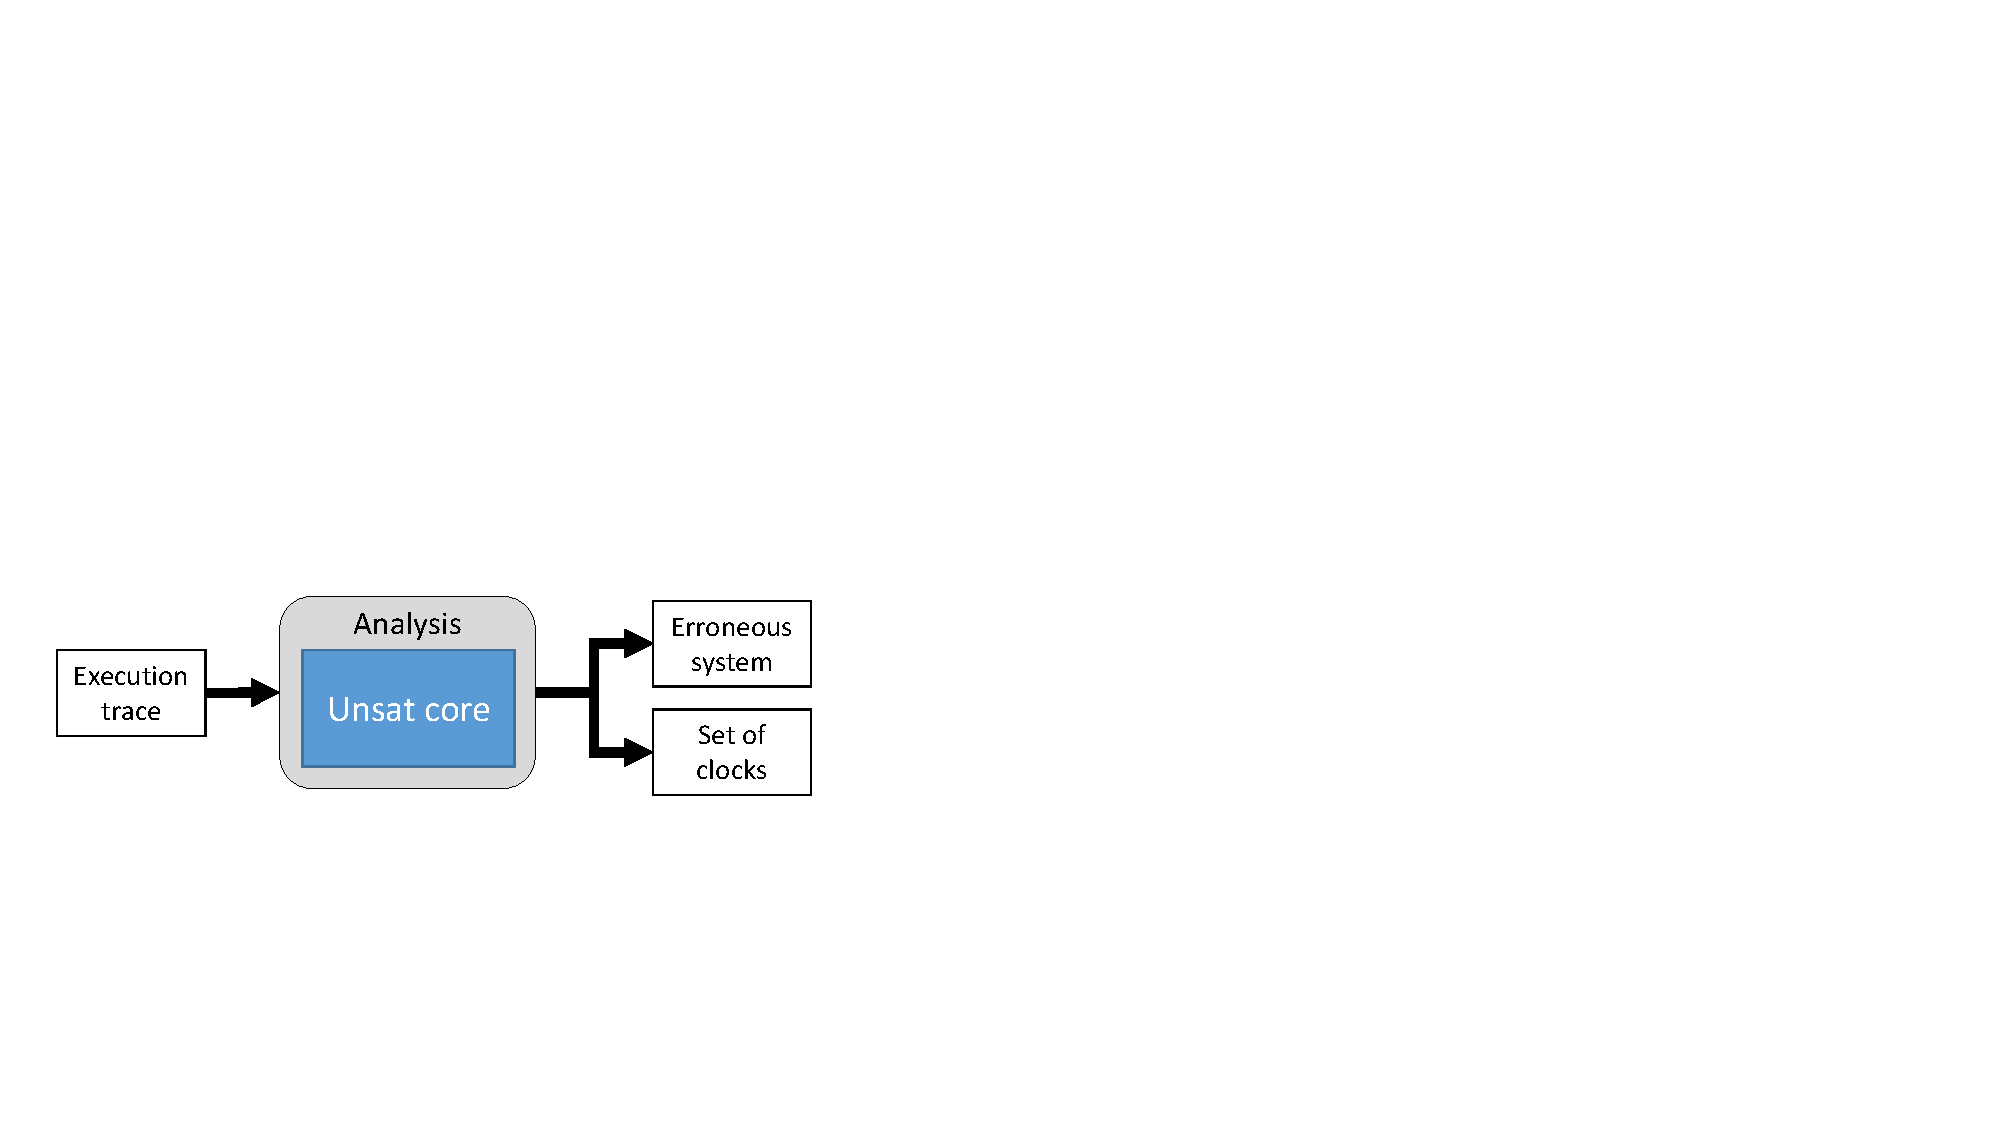
\includegraphics[width=.7\textwidth]{include/figures/modules_ta_anal}
	%\caption{Statespace-based refinement}
	%\label{fig:cegarssp}
\end{figure}

Solvers can be useful, not only to decide if a given set of constraints is satisfiable, but also -- if the answer is that the formula is unsatisfiable -- solvers have various features to show why they can not be satisfied. One of the possible helpful feature is deriving the so called \emph{unsat core} -- that is, a minimal (not necessarily minimum\footnote{A minimal unsat core does not guarantee that it is the smallest possible unsatisfiable subset of the given constraints, i.e. minimum. It only guarantees that the removal of any constraint would result in a satisfiable formula.}) set of the given constraints that is unsatisfiable in itself. This set of constraints can be used to determine the set of clock variables with what the current abstraction of the automaton has to be extended. In order to define the refinement set, the variables appearing in the unsat core have to be transformed back to the original variables. The set of original variables appearing in the constraints is the result of the algorithm.


\begin{runningExample}
	The result of checking satisfiability of $\varphi$ is \emph{No}, and the unsat core is $\varphi_{unsat}=x_1'=x_1+d_1 \wedge y_1'=y_1+d_1 \wedge x_1=0 \wedge y_1=0 \wedge x_1 \leq 10 \wedge x_1' \leq 10 \wedge y_1' \geq 20$. This means the automaton has to be refined with both $x$ and $y$ so that the spurious counterexample is eliminated.
\end{runningExample}

\subsubsection{Automaton refinement}

\begin{figure}[h]
	\centering
	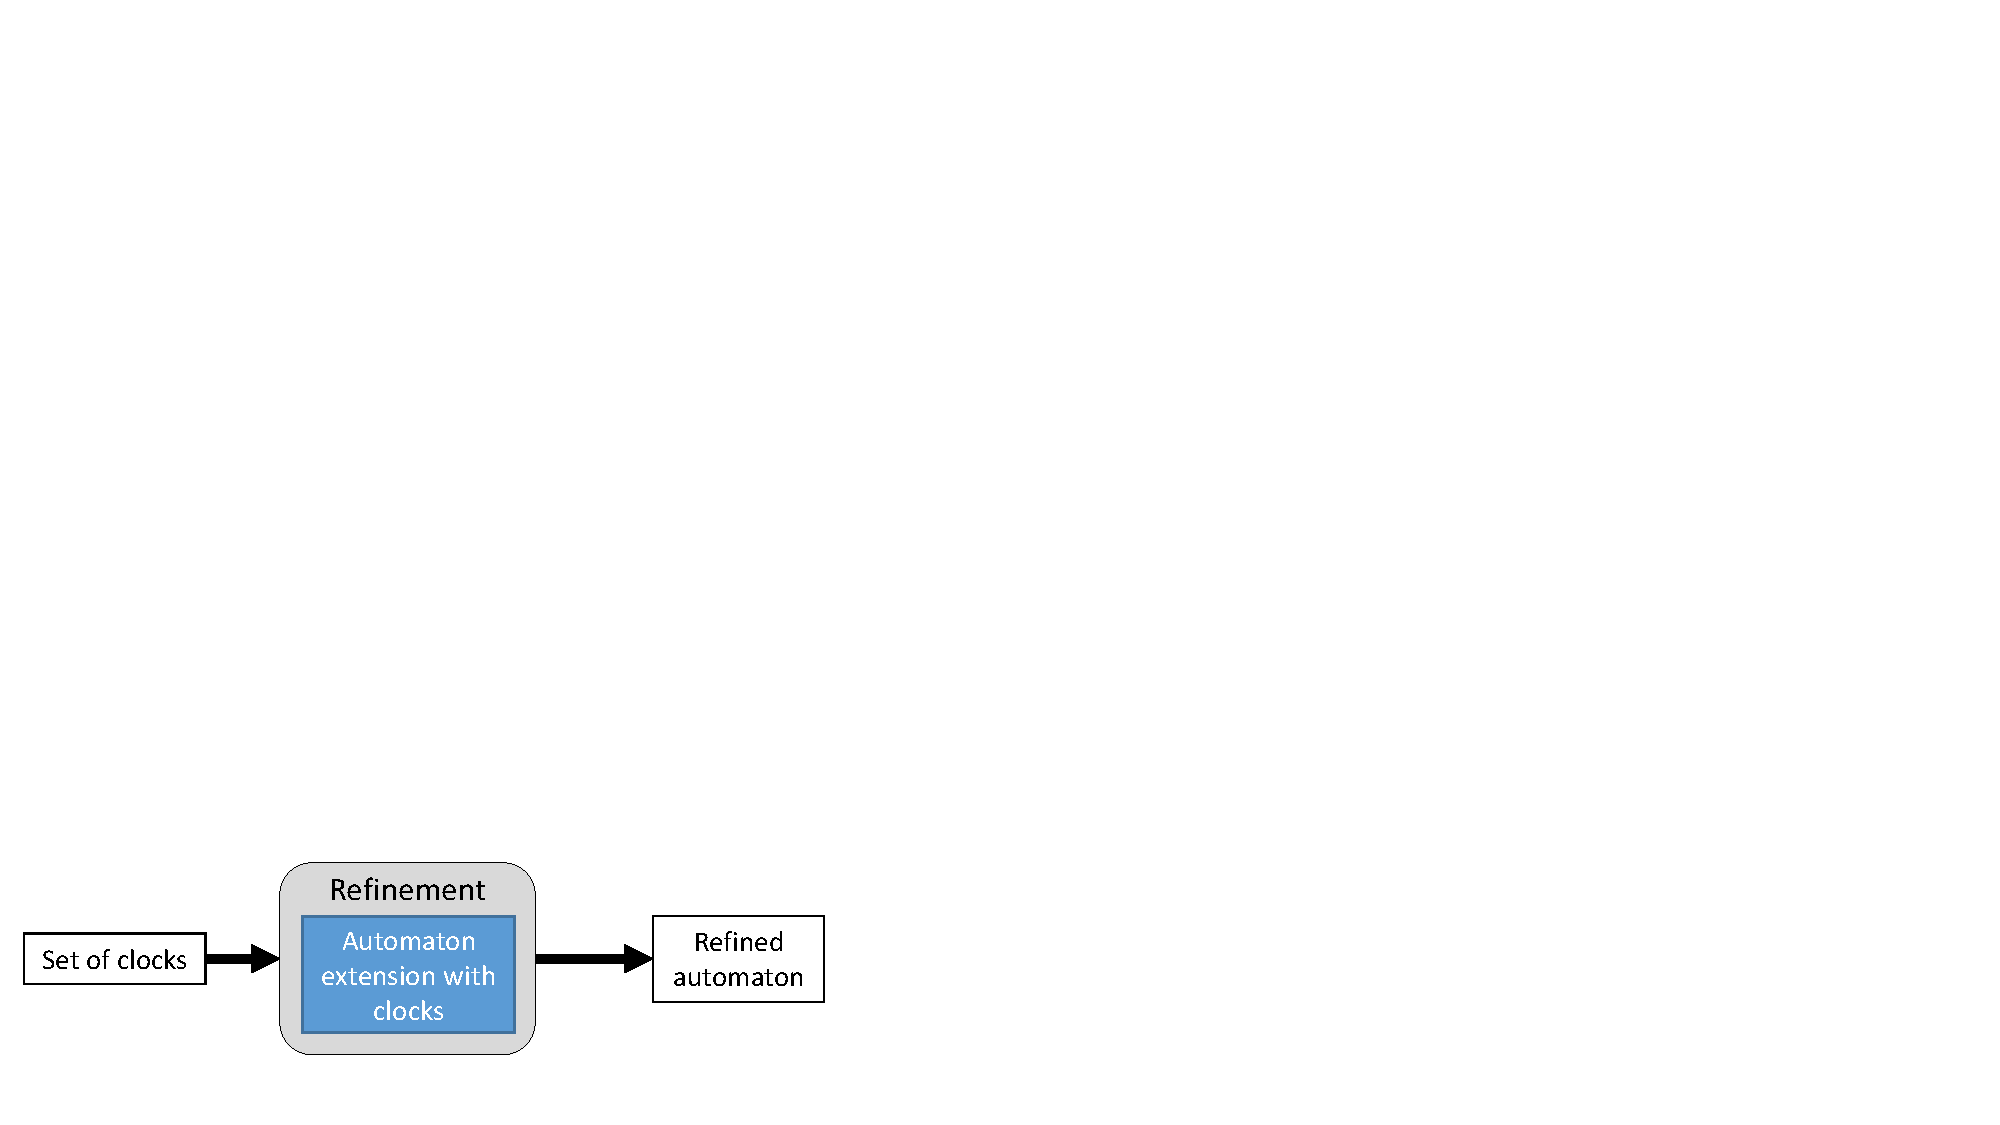
\includegraphics[width=.7\textwidth]{include/figures/modules_ta_ref}
	%\caption{State space-based refinement}
	%\label{fig:cegarssp}
\end{figure}

Given an original automaton $\mathcal{A}$ an abstract automaton $\mathcal{A'}$ and a set of clock variables to be added $C \subseteq \mathcal{C}$, the task is to refine $\mathcal{A'}$ so that each clock $c \in C$ appears in it. The task is to decide which of the guards, resets and invariants to include. Resets are easy to add: the ones that reset clocks in $C$ should be included, others don't. Guards and invariants are clock constraints -- conjunctive formulae of atomic constraints bounding the value of the clocks or the difference of two clocks. Decision can be made for each atomic formula one by one: those in which only clocks in $\mathcal{A'}$ or $C$ appear -- that is, difference constraints are only included if both clocks appear in $\mathcal{A'}$ or $C$.

\subsection{State space-based refinement}

\begin{figure} 
	\centering
	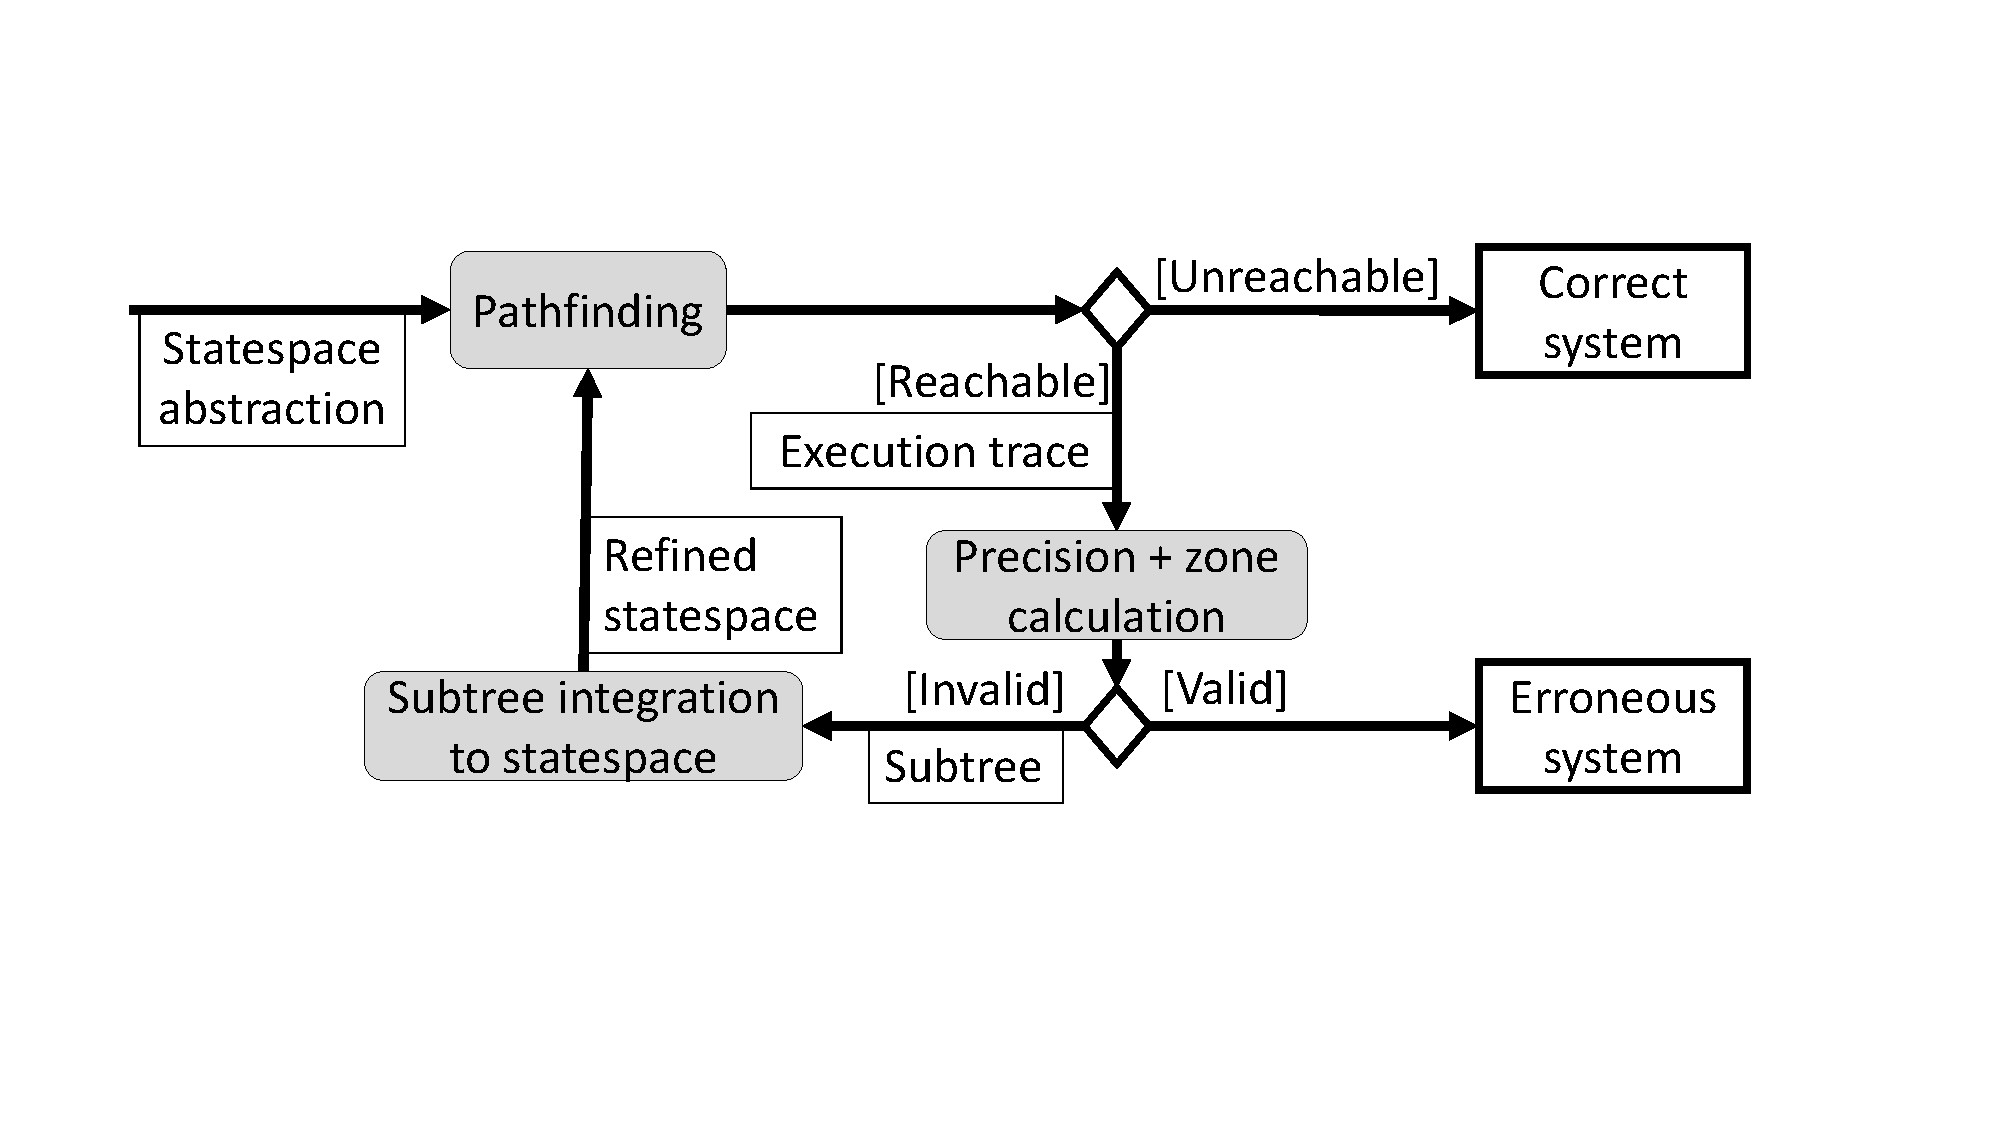
\includegraphics[width=.7\textwidth]{include/figures/alg_arch_ssp}
	\caption{State space-based refinement}
	\label{fig:cegarssp}
\end{figure}


In case of state space-based refinement, the representation of the state space has a defining role. In the proposed framework, the state space is represented by zone graphs -- this is common for all algorithms. However, the abstraction of the zone graph can be performed various ways. In this framework, the main idea is to explore the state space without considering clock variables (and in some cases discrete variables, too), and to refine the state space -- trace by trace -- by deciding which of the clock variables to include for each of the zones on that path. After that the graph is refined (clocks are included in the zones), and during the refinement it turns out whether the counterexample is feasible or not. Figure \ref{fig:cegarssp} depicts the architecture of this approach.

Because of the different approaches of abstraction, constructing the initial abstraction is not as straightforward as it was in case of automaton-refinement. All that can be said is that it is some sort of abstraction of the state space derived from the automaton without including clock variables.

The task of the model checking phase is to find a path from the initial location to the error location in the current abstraction of the zone graph. Because of this, the model checking phase of state space-based refinement is performed by pathfinding algorithms.

The task of the analysis phase can be divided into two parts:  decide which of the clock variables to include in the zones (i.e. the \emph{precision} of the zone) and calculate the zones on the trace (up to the given precision) and find out if it is feasible or not. 

When performing the first part it is important to find precisions (that might change along the trace) that is not too big (does not include too much variables) to be calculated efficiently, but includes all variables that are necessary to find out if he trace is feasible or not. The result of this part should be a function $P: V(G) \to 2^\mathcal{C}$ assigning precisions to the nodes of the current abstraction of zone graph.

As for the second part, calculating the correct zones can be performed by the steps of the algorithm presented in Section \ref{sec:tareach} with some modifications that help with handling the changes of precision along the zones in counterexample. If the error location is unreachable, a guard or invariant will eventually prove to one of the edges on the trace that it represents a transition that is not enabled.

The task of the refinement phase is to modify the current abstraction of the zone graph according to the states calculated in the analysis phase.

\begin{algorithm}
	\KwIn{$\mathcal{A}=\langle L,l_0,E,I \rangle$, $l_{err} \in L$}
	\KwOut{$\sigma=l_0 \xrightarrow{t_0} l_1 \xrightarrow{t_1} \cdots \xrightarrow{t_n} l_{err}$ if $l_{err}$ is reachable, \emph{No} otherwise}
	\BlankLine
	$\mathcal{G} \leftarrow$ inital($\mathcal{A}$) \tcc*{initial abstraction}
	\While{\emph{true}}{
		$\sigma \leftarrow$ path($\mathcal{G},l_0,l_{err},\mathcal{A}$) \tcc*{model checking}
		\eIf(\tcc*[f]{no counterexample is found}){$\not\exists \sigma$}
		{\KwRet{\emph{No}}\tcc*{unreachable}}
		{$P \leftarrow$ prec($\mathcal{A},\sigma$)  \;
		 $T \leftarrow$ calculateTrace($\sigma,P$) \tcc*{analysis}
			\eIf(\tcc*[f]{feasible trace}){$\exists \langle l_{err},z\rangle \in$ nodes($T$) for some $z \neq \emptyset$}{\KwRet{$\sigma$} \;}
			{$\mathcal{G} \leftarrow$ refine($\mathcal{G},T$)\tcc*{state space is refined accoring to $T$}}
		}
	}
	\caption{State space-based refinement} \label{alg:cerarssp}
\end{algorithm}

Algorithm \ref{alg:cerarssp} provides pseudocode for the described approach. Function \emph{initial}, \emph{path} and \emph{refine} are state space representation-dependent. Functions \emph{prec()},  and \emph{calculateTrace()} are components that can be chosen from the techniques described in the following sections, where two abstractions of the zone graph are presented, and algorithms are shown, mentioning the state space representation-dependent behaviours of model checking and refinement. Only those of the presented techniques can be used interchangeably, that are defined for the same representation.


%\section{Modules}
%This section describes the algorithms that can be used in the previously defined CEGAR realizations. Methods for automaton-based refinement are explained: model checkers, an algorithm for calculating the set of clock variables to refine the automaton, and the general algorithm for performing the refinement. Two possible representations of the abstract zone graph are presented. 
%Algorithms are presented on the automaton in Figure \ref{fig:loopinfinite} with $l_{err}=\text{\emph{end}}$ to ease understanding. From now on $\mathcal{A}$ will refer to that particular timed automaton.
%\subsection{Implementations for state space-based refinement}



\subsubsection{Graph representation}

The first representation of the abstract zone graph is another zone graph, with zones of varied precisions. To avoid confusion, from now on precisions of zones will always be shown: zones will be denoted by $z_{C}$ where $C \subseteq \mathcal{C}$ is the precision of the zone. Zones of the real zone graph (without abstraction) are denoted by $z_{\mathcal{C}}$.

A node $\langle l, z_{C} \rangle$ of the abstract zone graph can represent any nodes $\langle l, z_{\mathcal{C}}' \rangle$ of the real zone graph, that contains the same location $l$, and some zone $z'_{\mathcal{C}}$ for which $z'_C \subseteq z_C$ holds (where $z'_C$ means a spatial projection of $z_{\mathcal{C}}'$ to the subspace spanned by the clocks in $C$). This means $\langle l, z_{\emptyset} \rangle$ can represent any nodes of the real zone graph containing $l$. 

Based on this, the initial abstraction can be constructed by assigning a node $\langle l, z_{\emptyset} \rangle$ to each location $l \in L$. The graph can then be completed with edges: for each $e=(l,g,r,l') \in E$ a new edge of the zone graph should be included pointing from $\langle l, z_{\emptyset} \rangle$ to $\langle l', z_{\emptyset} \rangle$.

\begin{figure}
	\centering
	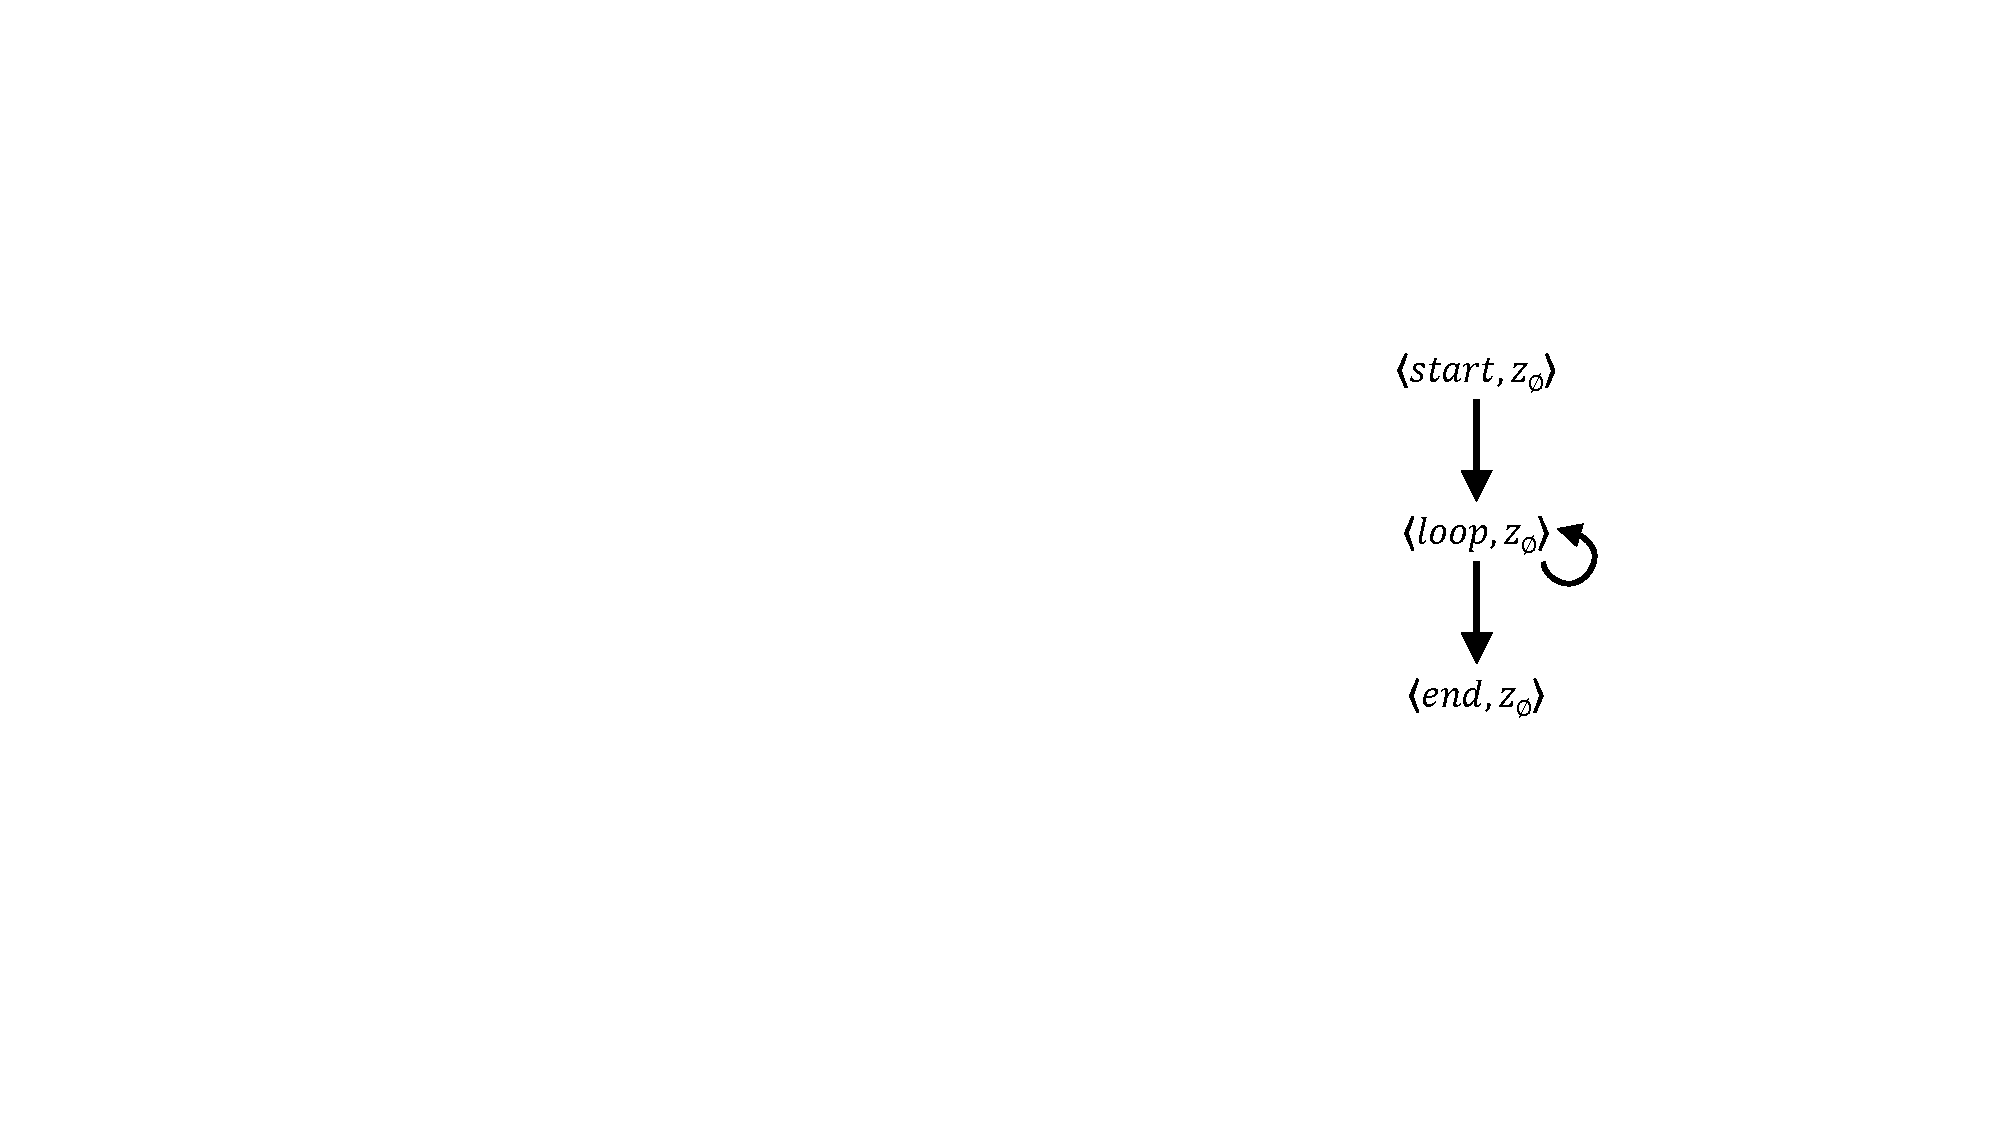
\includegraphics[width=.2\textwidth]{include/figures/graph_init}
	\caption{Initial abstraction of $\mathcal{A}$}
	\label{fig:graphinit}
\end{figure}

\begin{runningExample}
	The initial abstraction for $\mathcal{A}$ is depicted in Figure \ref{fig:graphinit}.
\end{runningExample}

During the algorithm this graph will be refined by the zones calculated in the refinement phase. Sometimes nodes will get replicated, or edges deleted (the precise algorithm will be described later), but it will remain  an abstraction of the concrete zone graph. 

%Discrete valuations are also calculated in the refinement phase.


 
% It is common in both representations that the abstraction of the nodes is based on a set of clocks (precision) to include -- just like in case of the automaton-based refinement. In the initial abstraction no clocks are included in any of the nodes

\subsubsection{Tree representation}
The other representation of the abstract zone graph is based on the idea of search trees. Instead of keeping track of the full (abstract) zone graph (like we did with the other representation) details of the tree will be uncovered in the model checking phase of the CEGAR loop. However, one thing is common in both representations:  the abstraction of the nodes is based on a set of clocks (precision) to include (just like in case of the automaton-based refinement) and initially all precisions are empty. The state space exploration will also operate on empty precision sets, and the zones will be calculated in the refinement phase. In this case, discrete valuations can be calculated during state space exploration (but it is not necessary).

Let us define the formalism to represent the abstract tree.

\begin{dfn}
	The auxiliary graph can be defined as a tuple $\langle N_e, N_u, E^\uparrow, E^\downarrow \rangle$ where
	\begin{itemize}
		\item $N_e \subseteq L \times \mathcal{B}(\mathcal{C})$ is the set of explored nodes,
		\item $N_u \subseteq L \times \mathcal{B}(\mathcal{C})$  is the set of unexplored nodes,
		\item $E^\uparrow \subseteq (N_e \times N)$, where $N = N_e \cup N_u$ is the set of upward edges and
		\item $E^\downarrow \subseteq (N_e \times N)$  is the set of downward edges.
	\end{itemize}
	 The sets $N_e$ and $N_u$ as well as the sets $E^\uparrow$ and $E^\downarrow$ are disjoint. $T^\downarrow=(N,E^\downarrow)$ is a tree.
\end{dfn}
 %The depth of a node $n$ in $T$ is denoted by $d(n)$.
 
Nodes are built from a location and a zone like in the zone graph but in this case nodes are distinguished by their trace leading to them from the initial node. This means the graph can contain multiple nodes with the same zone and the same location, if the represented states can be reached through different traces. The root of $T$ is the initial node of the (abstract) zone graph. A downward edge $e$ points from node $n$ to $n'$ if $n'$ can be reached from $n$ in one step in the zone graph. %In this case $d(n')=d(n)+1$.

Upward edges are used to collapse infinite traces of the representation, when the states are explored in former iterations. An upward edge from a node $n$ to a previously explored node $n'$ means that the states
represented by $n$ are a subset of the states represented by $n'$, thus it is unnecessary to keep searching for a
counterexample from $n$, because if there exists one, another one will exist
from $n'$. Searching for new traces is only continued on nodes without an upward edge. This way, the graph can be kept finite, unless the discrete variables of the automaton prevent it.

Initially, the graph contains only one, unexplored node $\langle l, z_{\emptyset} \rangle$, and as the state space is explored, unexplored nodes become explored nodes, new unexplored nodes and edges appear, until a counterexample is found. During the refinement phase zones are calculated, new nodes and edges appear and complete subtrees disappear. State space exploration will then be continued from the unexplored nodes, and so on. Discrete valuation can be calculated during state space exploration.

\begin{runningExample}
	The initial abstraction for $\mathcal{A}$ is a single unexplored node $n_0=\langle \textit{start}, z_{\emptyset} \rangle$.
\end{runningExample}


\subsubsection{State space exploration}

\begin{figure}[h]
	\centering
	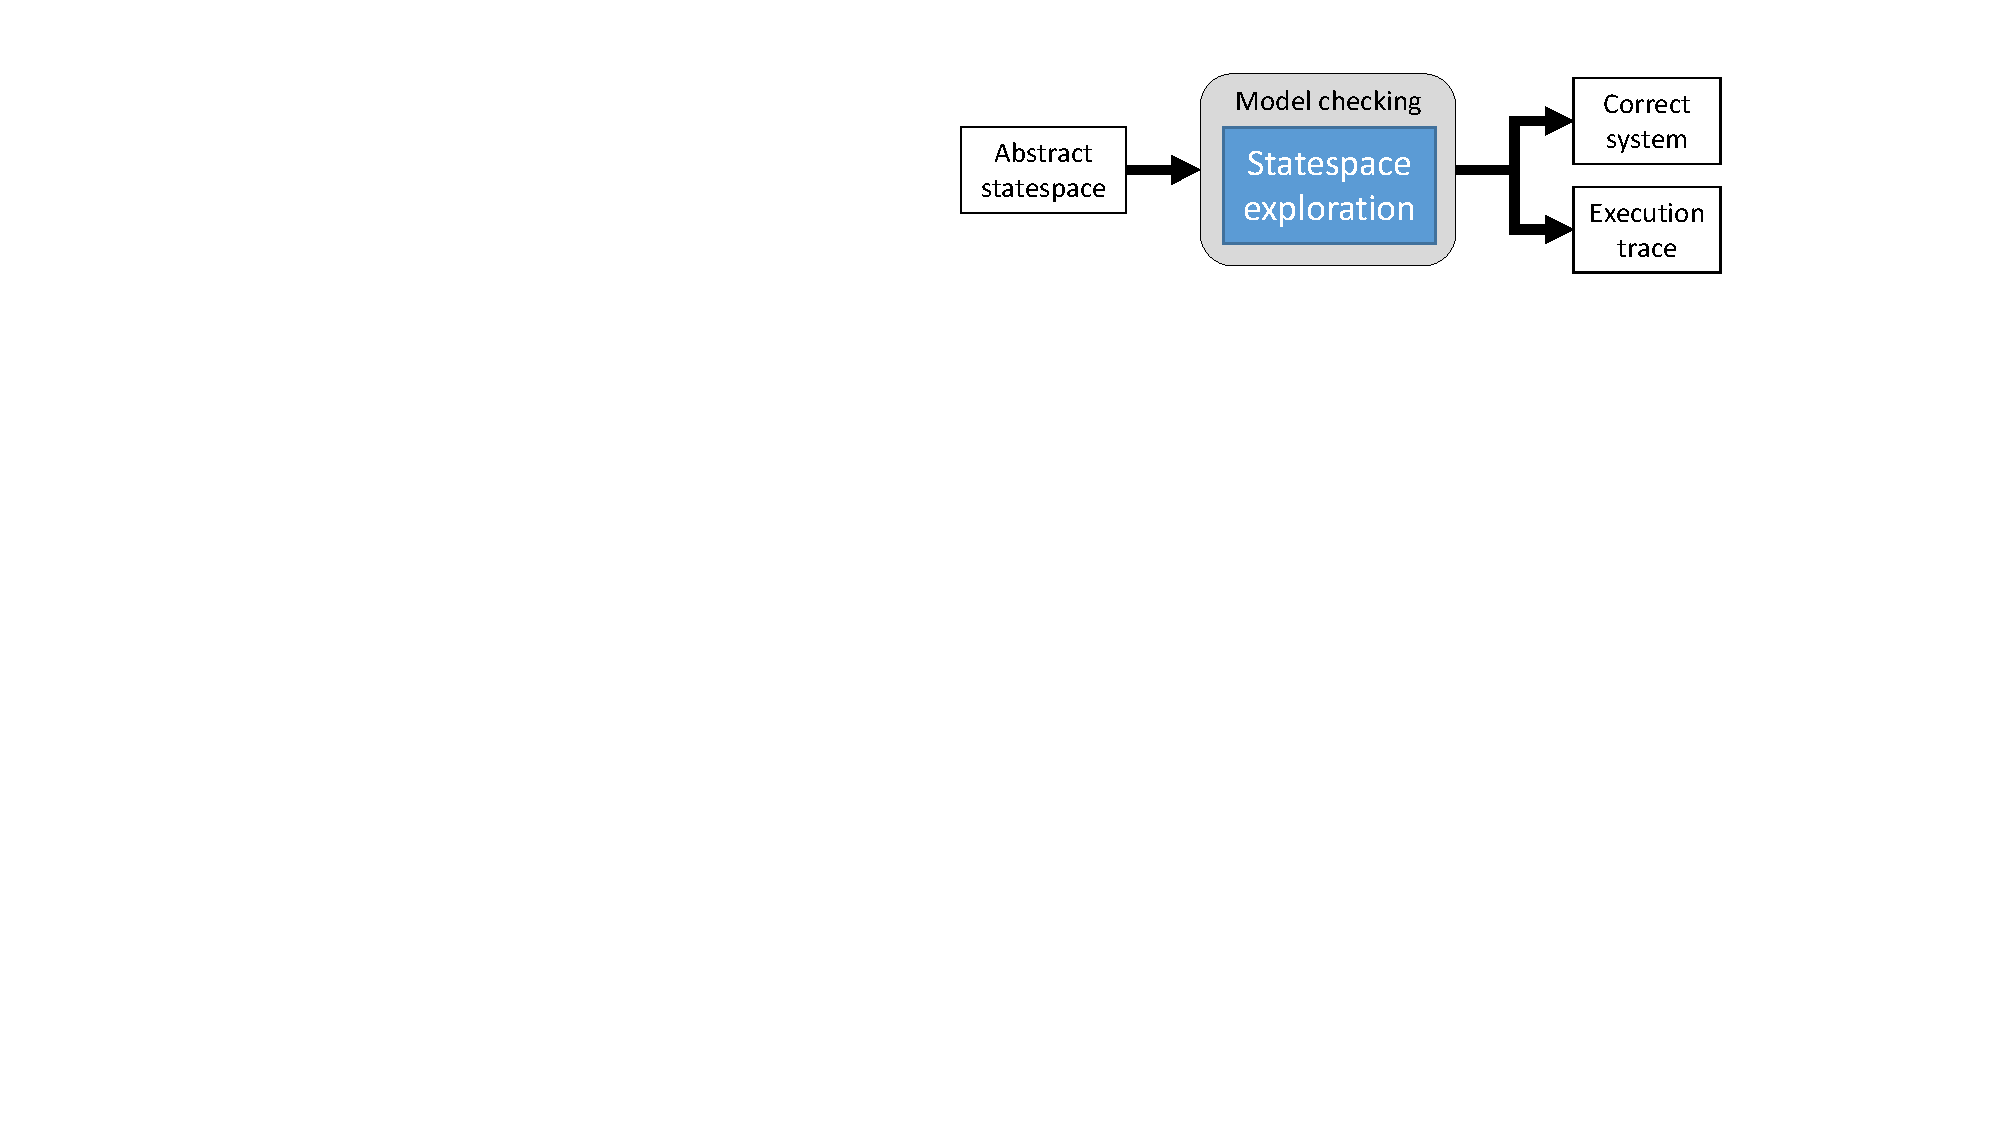
\includegraphics[width=.7\textwidth]{include/figures/modules_ssp_mc}
	%\caption{State space-based refinement}
	%\label{fig:cegarssp}
\end{figure}

The task of the model checking phase is to find traces from $l_0$ to $l_{err}$. In case of the graph representation, where $l_{err}$ appears in the node  $\langle l_{err}, z_{\emptyset} \rangle$ even in the initial abstraction, model checking becomes a pathfinding problem from $\langle l_{0}, z_{\emptyset} \rangle$ to $\langle l_{err}, z_{\emptyset} \rangle$ in the abstract zone graph. This can be performed by any pathfinding algorithm.

\begin{runningExample}
	Pathfinding in $\mathcal{A}$'s initial abstraction finds the previously mentioned counterexample $\sigma= \text{\emph{start}} \to \text{\emph{loop}} \to \text{\emph{end}}$.
\end{runningExample}

In case of the tree representation, $l_{err}$ does not appear in the graph and the state space exploration has to be continued until a node $\langle l_{err}, z_{\emptyset} \rangle$ appears. State space exploration has to be performed the following way.

In each iteration a node $n=\langle l, z_{C} \rangle \in N_u$ for some $C$ is chosen. First, it is checked if the states $n$ represents are included in some other node $n'=\langle l, z'_{C} \rangle$ with a zone of the same precision. If this is the case an upward edge is introduced from $n$ to $n'$ and $n$ becomes explored. Otherwise, $n$ has yet to be explored. For each outgoing edge $e(l,g,r,l')$ of $l$ in the automaton a new unexplored node $\langle l, z_{\emptyset} \rangle$ is introduced with an edge pointing to it from $n$, which becomes explored. If any of the new nodes contains $l_{err}$, the algorithm terminates. Otherwise, another unexplored node is chosen, and so on.

\begin{runningExample}
	Exploration of $\mathcal{A}$'s abstract state space starts by exploring $n_0$, that is performed by introducing a new (unexplored node) $n_1=\langle \text{\emph{loop}}, z_\emptyset \rangle$ with a downward edge $n_0 \to n_1$. The erroneous location is not explored yet so the iteration continues. Location \emph{loop} has two outgoing edges. The loop edge introduces $n_2=\langle \text{\emph{loop}}, z_\emptyset \rangle$ with a downward edge $n_1 \to n_2$. Edge \emph{loop} $\to$ \emph{end} introduces $n_3=\langle \text{\emph{end}}, z_\emptyset \rangle$ with $n_1 \to n_3$. The erroneous location is found and $\sigma= n_0 \to n_1 \to n_3$ is proposed as a counterexample.
\end{runningExample}

\begin{algorithm}
	\KwIn{$\mathcal{T}=\langle N_e, N_u, E^\uparrow, E^\downarrow \rangle$, $l_{err}, \mathcal{A}$}
	\KwOut{$\sigma=l_0 \xrightarrow{t_0} l_1 \xrightarrow{t_1} \cdots \xrightarrow{t_n} l_{err}$ if $l_{err}$ is reachable in the abstract statespace, \o\ otherwise}
	\BlankLine
	\For{$n=\langle l,z_C \rangle \in N_u$}{
		newnodes $\leftarrow \emptyset$ \tcc*{set of successor nodes}
		$N_u \leftarrow N_u \setminus \{n\}$ \;
		$N_e \leftarrow N_e \cup \{n\}$ \tcc*{node marked as explored}	
		\eIf(\tcc*[f]{$n'$ contains all states of $n$}){$\exists n'=\langle l,z'_C \rangle \in N_e$ such that $z_C \subseteq z'_C$}
		{ $E^\uparrow \leftarrow E^\uparrow \cup \{(n,n')\}$ \;}
		{\For{$e=(l,a,g,l') \in E(\mathcal{A})$}{
				$n' \leftarrow \langle l',z_\emptyset \rangle$ \;
				newnodes $\leftarrow$ newnodes $\cup \{n'\}$ \;
				$N_u \leftarrow N_u \cup \{n'\}$ \;	
				$E^\downarrow \leftarrow E^\downarrow\cup \{(n,n')\}$ \;
		}
		}
		\If(\tcc*[f]{$l_{err}$ reached}){$\exists n'=\langle l_{err}, z_\emptyset\rangle \in$ newnodes}{\KwRet{trace($n'$)}\;}
	}
	\KwRet{\o} \tcc*{$l_{err}$ is unreachable}
	\caption{An implementation of of function \emph{path}} \label{alg:path}
\end{algorithm}

Algorithm \ref{alg:path} provides pseudocode for the presented method. Function \emph{trace} calculates the sequence of downwards arrows through wich the node is reached from the root of $\mathcal{T}$. 

\subsubsection{Trace activity-based precision calculation}

\begin{figure}[h]
	\centering
	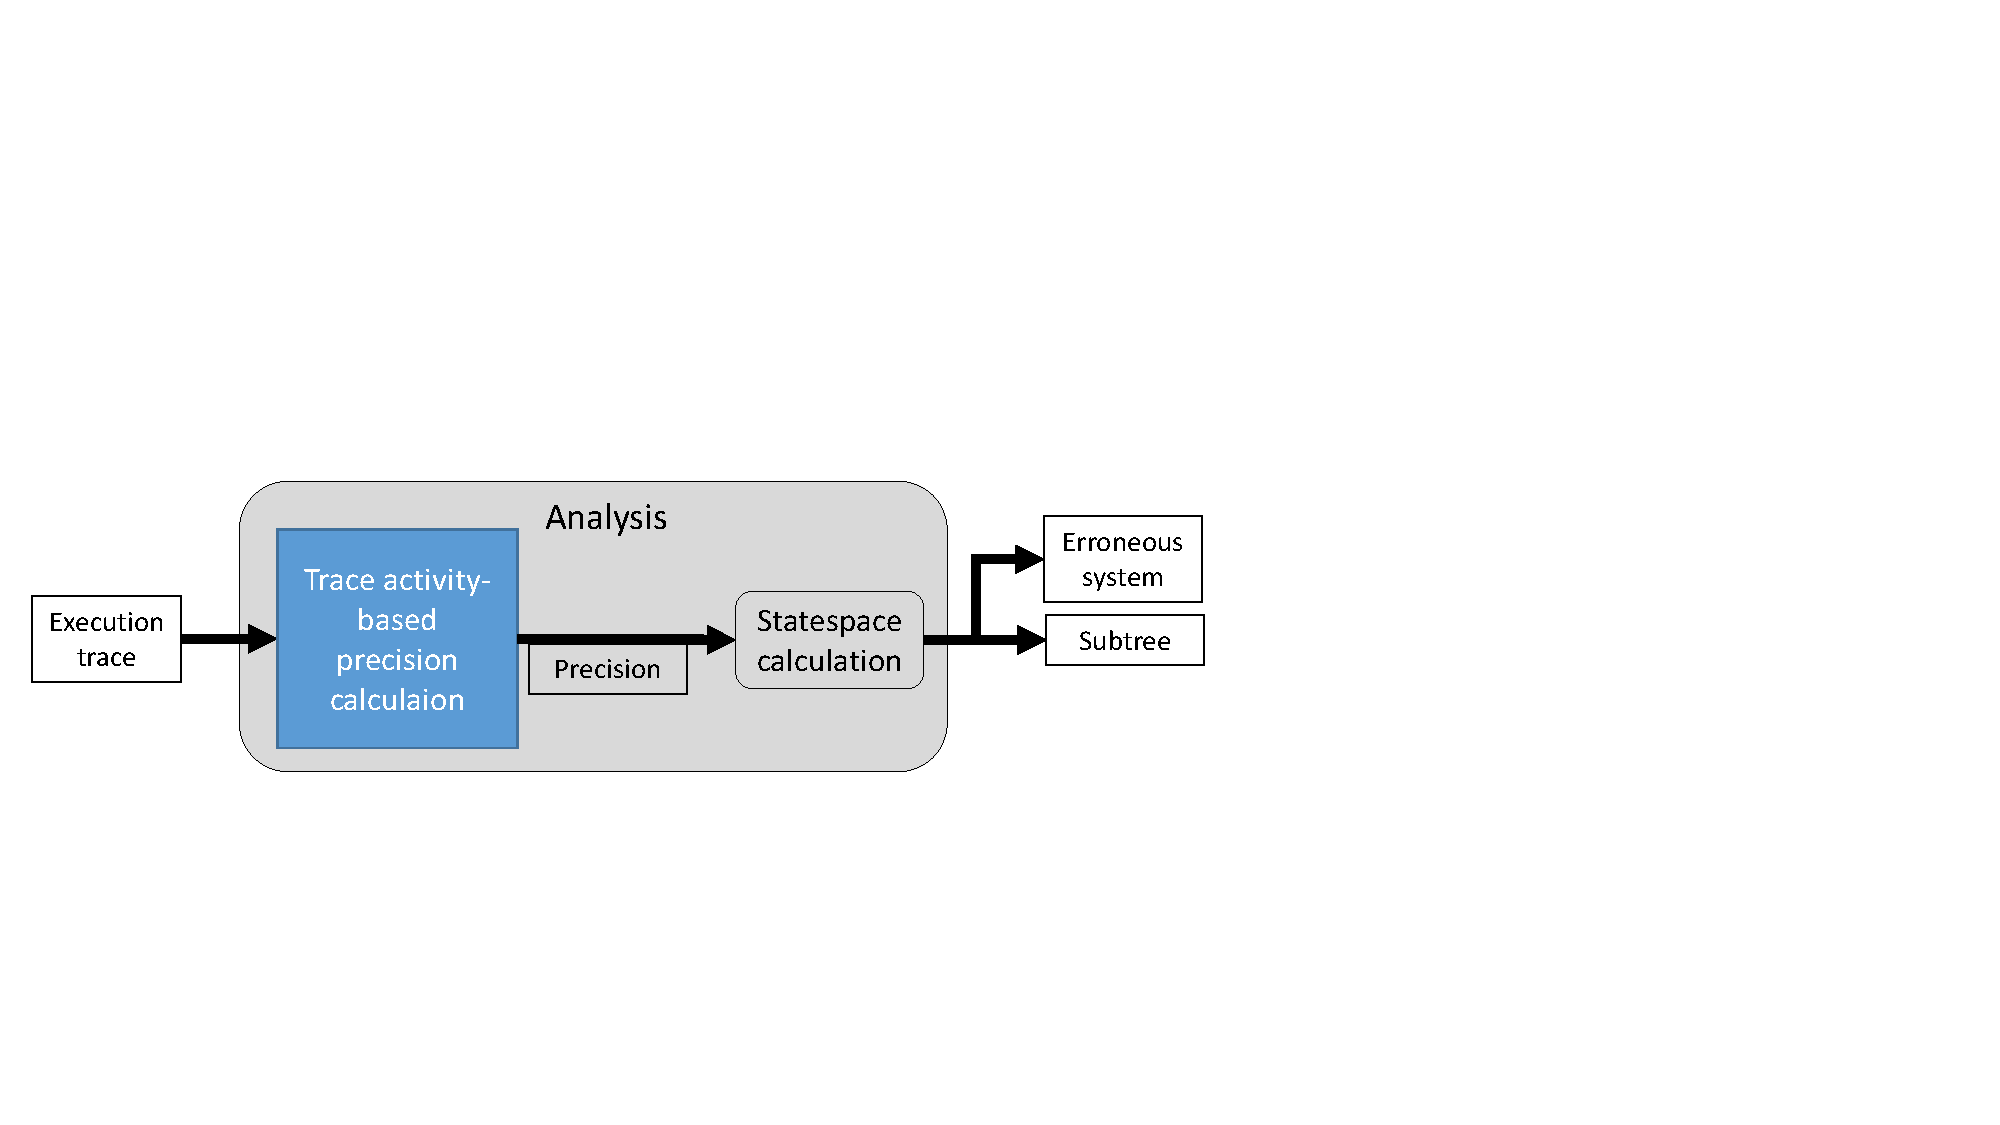
\includegraphics[width=\textwidth]{include/figures/modules_ssp_anal_act}
	%\caption{Statespace-based refinement}
	%\label{fig:cegarssp}
\end{figure}

The task of the analysis phase is to determine the precision of each zones on a given counterexample. The abstraction \emph{activity} as described in Section \ref{sec:acitivity} is able to assign a set of clocks for each locations of the automaton, without affecting its behaviour. Assigning $act(l)$ for each node $n=\langle l, z_{C} \rangle$ would be a good solution of the task, however it can be made more efficient by considering the fact that we are only examining an execution trace, and we only need to know if it is feasible.

Based on \emph{activity} a new abstraction can be introduced, called \emph{trace activity} $Act_\sigma(n): N \to 2^\mathcal{C}$ which does the same thing as activity, except for a trace: it assigns precisions to nodes (not locations in this case, because the same location may appear multiple times ion a trace with different activity). The algorithm calculating trace activity operates the following way.

The algorithm iterates over the counterexample trace, but backwards. In the final node  $n_{err}=\langle l_{err}, z_{\emptyset} \rangle$ it is not important to know the valuations, as the only important thing to know if it is reachable. Therefore $Act_\sigma(n_{err})=\emptyset$. After that $Act_\sigma(n_i)$ can be calculated from $Act_\sigma(n_{i+1})$ and the edge $e_i(l_i,g_i,r_i,l_{i+1})$ used by transition $t_i$. Since $r_i$ resets clocks, their values in $l_i$ will have no efficient on the systems behaviour in $l_{i+1}$. Thus clocks in $r_i$ can be excluded. It is necessary to know if $t_i$ is enabled, so $\textit{clk}(g_i)$ must be active in $n_i$. It is also important to satisfy the invariant of $l_i$ thus $\textit{clk}(I(l_i))$ must be included. This gives us the formula $Act_\sigma(n_i)=(Act_\sigma(n_{i+1}) \setminus r_i) \cup \textit{clk}(g_i) \cup \textit{clk}(I(l_i))$. 

\begin{runningExample}
	Calculating trace activity of $\sigma= n_0 \to n_1 \to n_3$ starts from the erroneous node $n_3$ by $Act_\sigma(n_3)=\emptyset$. Both $x$ and $y$ are reset on edge \emph{loop} $\to$ \emph{end} and only $y$ is tested, but $x$ appears in \emph{loop}'s invariant, thus $Act_\sigma(n_1)=\{x,y\}$. Since both clocks are reset on edge \emph{start} $\to$ \emph{loop}, $Act_\sigma(n_0)=\emptyset$.
\end{runningExample}

\subsubsection{Unsat core-based precision calculation}

\begin{figure}[h]
	\centering
	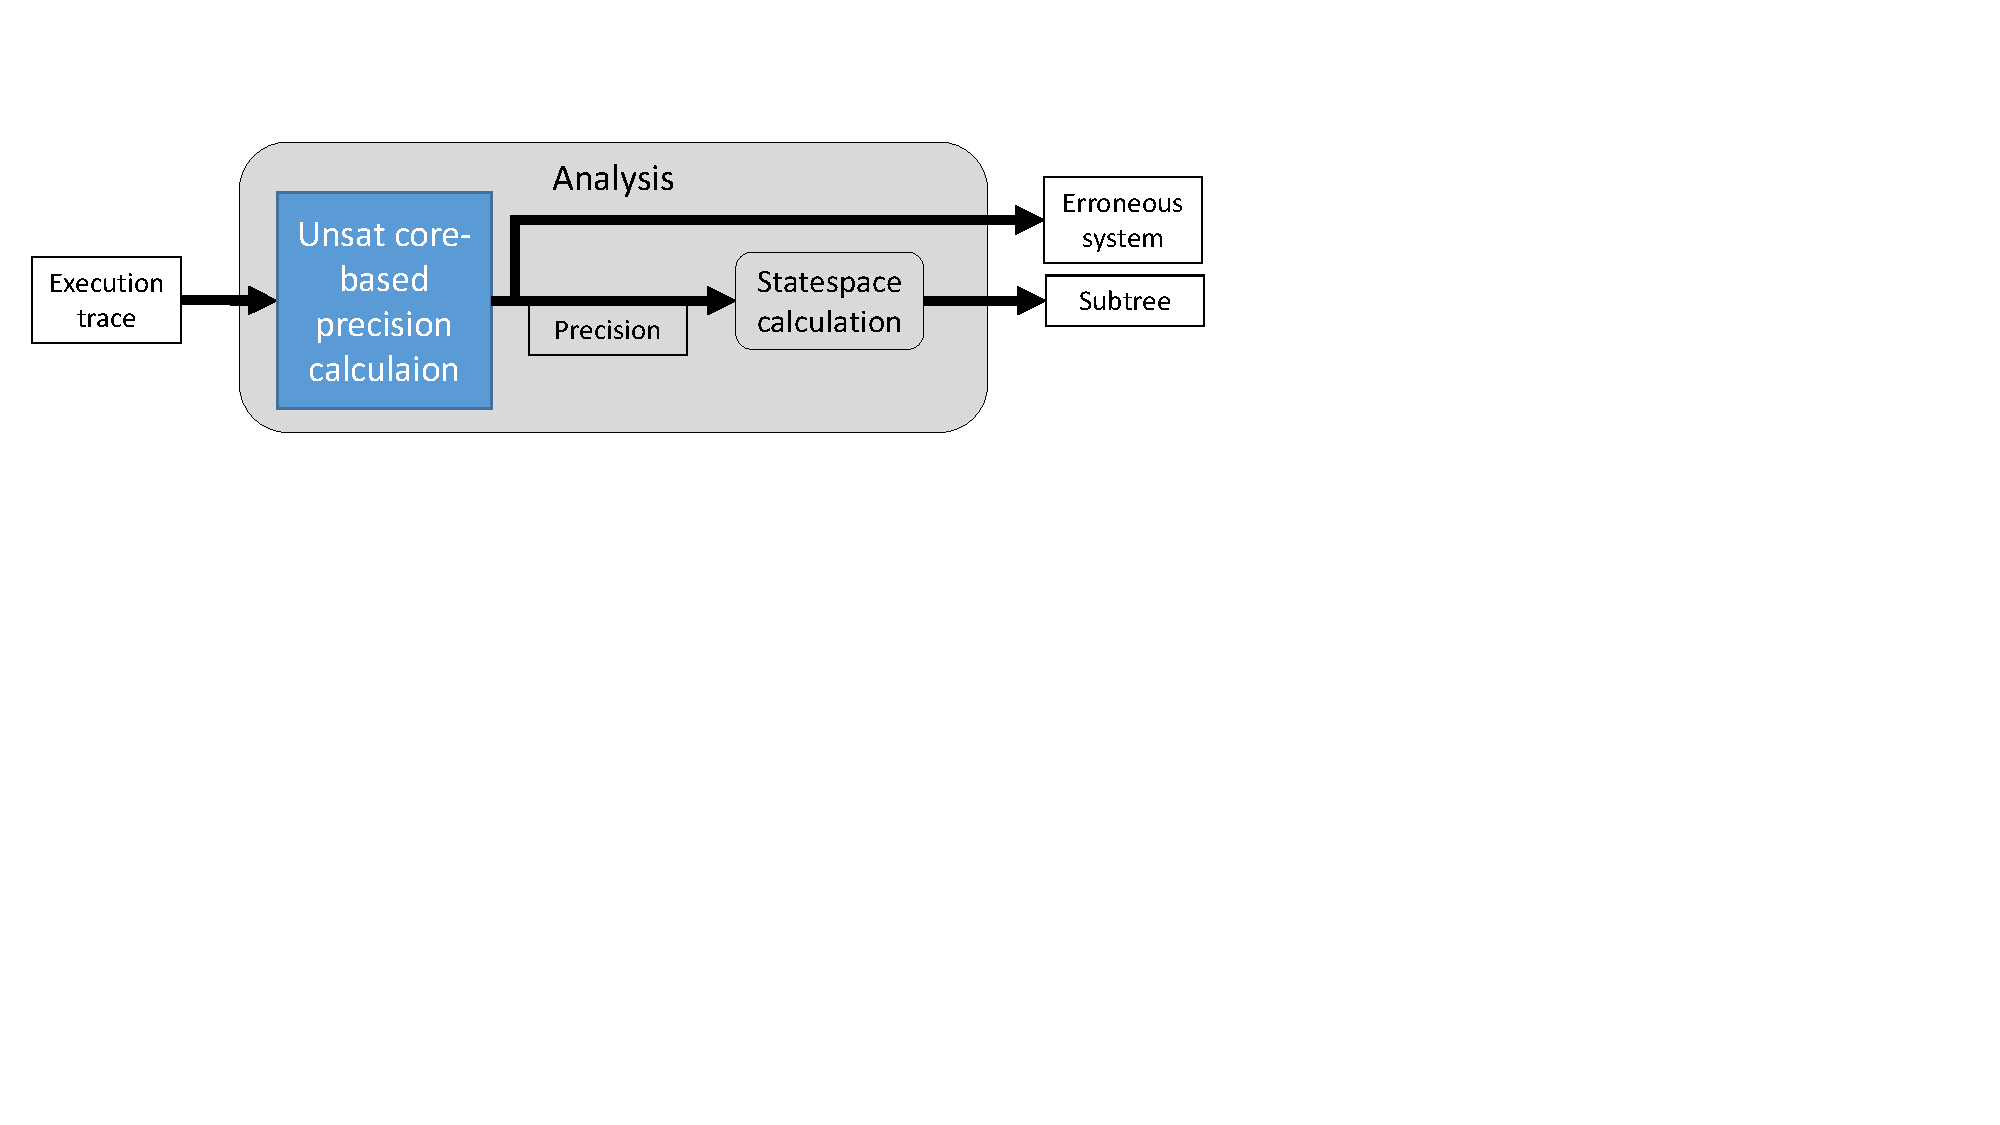
\includegraphics[width=\textwidth]{include/figures/modules_ssp_anal_uncore}
	%\caption{Statespace-based refinement}
	%\label{fig:cegarssp}
\end{figure}


Unsat core can also be used to determine the necessary precision of a given counterexample. First, the SMT formula described in Section \ref{sec:satmc} is checked by a solver. If it is satisfiable, the counterexample is feasible. Thus, there is no need to refine the graph, the CEGAR algorithm can terminate (or $\emptyset$ can be assigned to all nodes as a precision and the algorithm will terminate in the refinement phase). Otherwise, unsat core has to be examined. When constructing the SMT formula, variables were introduced for each step. Thus precision can be obtained from the unsat core by step: if $c_i$ or $c_i'$ appears in the unsat core $c$ must be included in the precision assigned to $n_i$.

\begin{runningExample}
	As it was mentioned, the unsat core of $\varphi$ is $\varphi_{unsat}=x_1'=x_1+d_1 \wedge y_1'=y_1+d_1 \wedge x_1=0 \wedge y_1=0 \wedge x_1 \leq 10 \wedge x_1' \leq 10 \wedge y_1' \geq 20$. The included variables representing clock variables are $x_1',x_1,y_1'$ and $y_1$. This results in precision $\emptyset$ for $n_0$, $\{x,y\}$ for $n_1$ and $\emptyset$ for $n_3$.
\end{runningExample}

\subsubsection{State space calculation}

\begin{figure}[h]
	\centering
	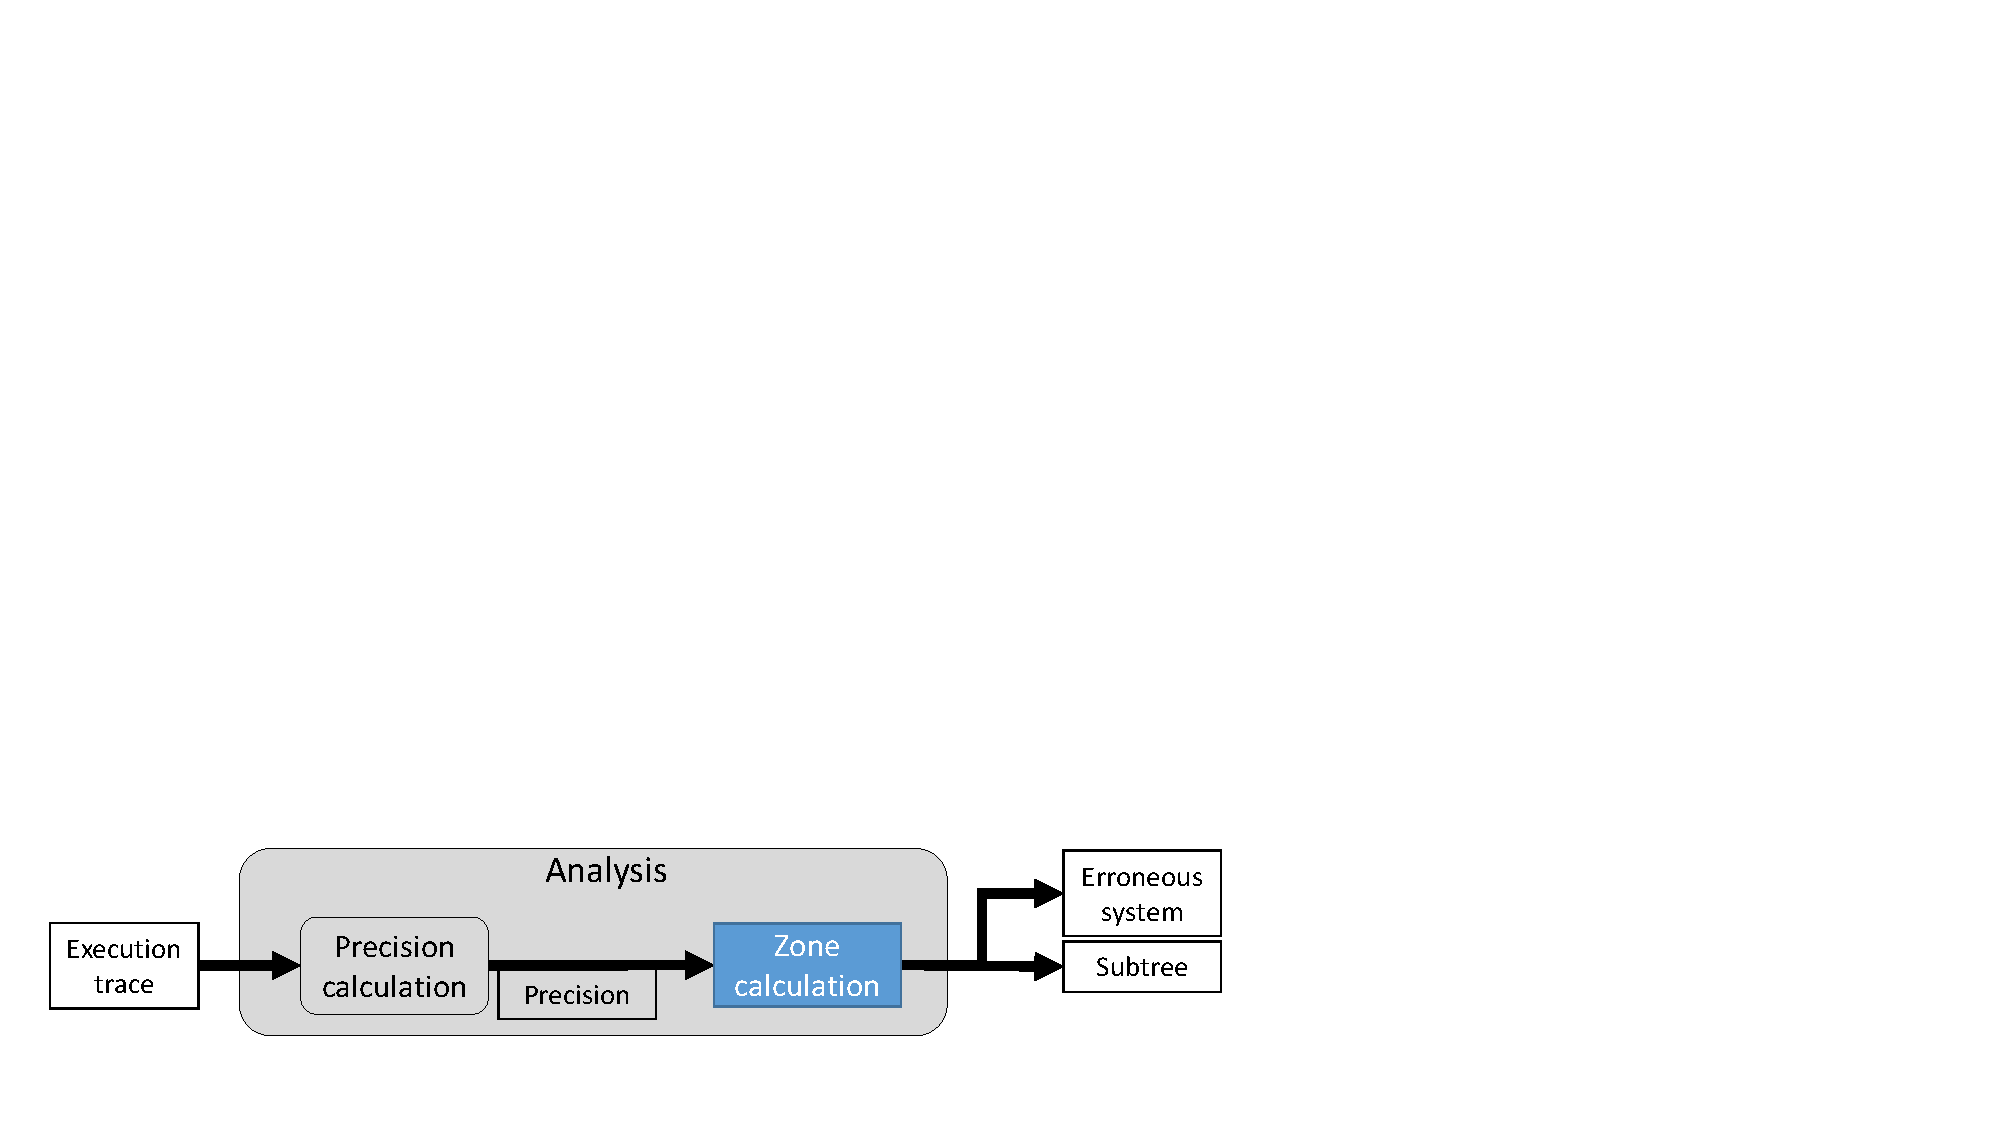
\includegraphics[width=\textwidth]{include/figures/modules_ssp_anal_zone}
	%\caption{Statespace-based refinement}
	%\label{fig:cegarssp}
\end{figure}


The task of the refinement phase is to assign correct zones of the given precision for each node in the trace. It is important to mention that the zones on the trace may already be refined to some precision $C'$ that is independent from the new precision $C$. In this case the zone has to be refined to the precision $C \cup C'$.  The initial zone can be calculated as described in Section \ref{sec:tareach}, except this time not all variables have to be included.  After that for each edge in the trace, the zone in the next node can be calculated with some little modifications of the corresponding part of the zone graph exploration algorithm regarding the precision change.

Assume the zone $z_i$ of node $n_i$ is refined to precision $C_i$ and the next zone $z_{i+1}$ in node $n_{i+1}$ has to be refined to $C_{i+1}$. Consider the DBM implementation of zones. Variables $C_{old}=C_{i} \setminus C_{i+1}$ have to be excluded from the precision. This can be done by performing \emph{free($c$)} for each $c \in C_{old}$, but in \cite{bengtsson2004timed} the operation \emph{free($c$)} only affects the row and the column belonging to $c$. Thus, for space saving purposes, the row and column of $c$ can simply be deleted from the DBM. 

Variables $C_{new}=C_{i+1} \setminus C_i$ have to be introduced. This is a more complex task, since the value is necessary to know. \emph{Trace activity} is constructed in a way that new clocks can only appear when they are reset. In this case, introducing the new variable is simple: add a new row and column to the DBM, belonging to $c$ and call \emph{reset($c$)}. However this is not always the case for \emph{unsat core}. It is possible that some constraints only appear in the unsat core, because they contradict each other, or a variable $c$ may appear in the unsat core, because several constraints combined can result in an unsatisfiable constraint that does not include $c$. 

\begin{example}
	Consider the automaton in Figure \ref{fig:splitex}. The unsat core-based precision of $S1$ is $\{x,y\}$, and $\{x,y,z\}$ of $S2$, but $z$ is not reset on $S1 \to S2$. In the unsat core it appears in $x < z+1$ and $z < y+1$ that imply $x < y+2$.
\end{example}

It is clear that in this case the concrete value of the variable $z$ doesn't matter, it is only there so that the constraints it appears in are considered. Because of this, there is no need to assign a precise value to $z$ -- introduce a row and a column belonging to $z$ and then call \emph{free($z$)}.

The correct zones on the trace are calculated. It is important to consider that sometimes the \emph{split()} operation results in more than one zones. In this case the corresponding node is replicated and one of the result zones is assigned to each versions of the node. Exploration has to be continued from that node, thus the refinement of a trace may result in a tree.

\begin{runningExample}
	The refinement of trace $\sigma$ results in $\langle \text{\emph{start}}, z_\emptyset \rangle \to \langle \text{\emph{loop}}, x=y \leq 10 \rangle$.
\end{runningExample}

%\todo{pszeudokód az eddigiekről}


\subsubsection{State space refinement}

\begin{figure}[h]
	\centering
	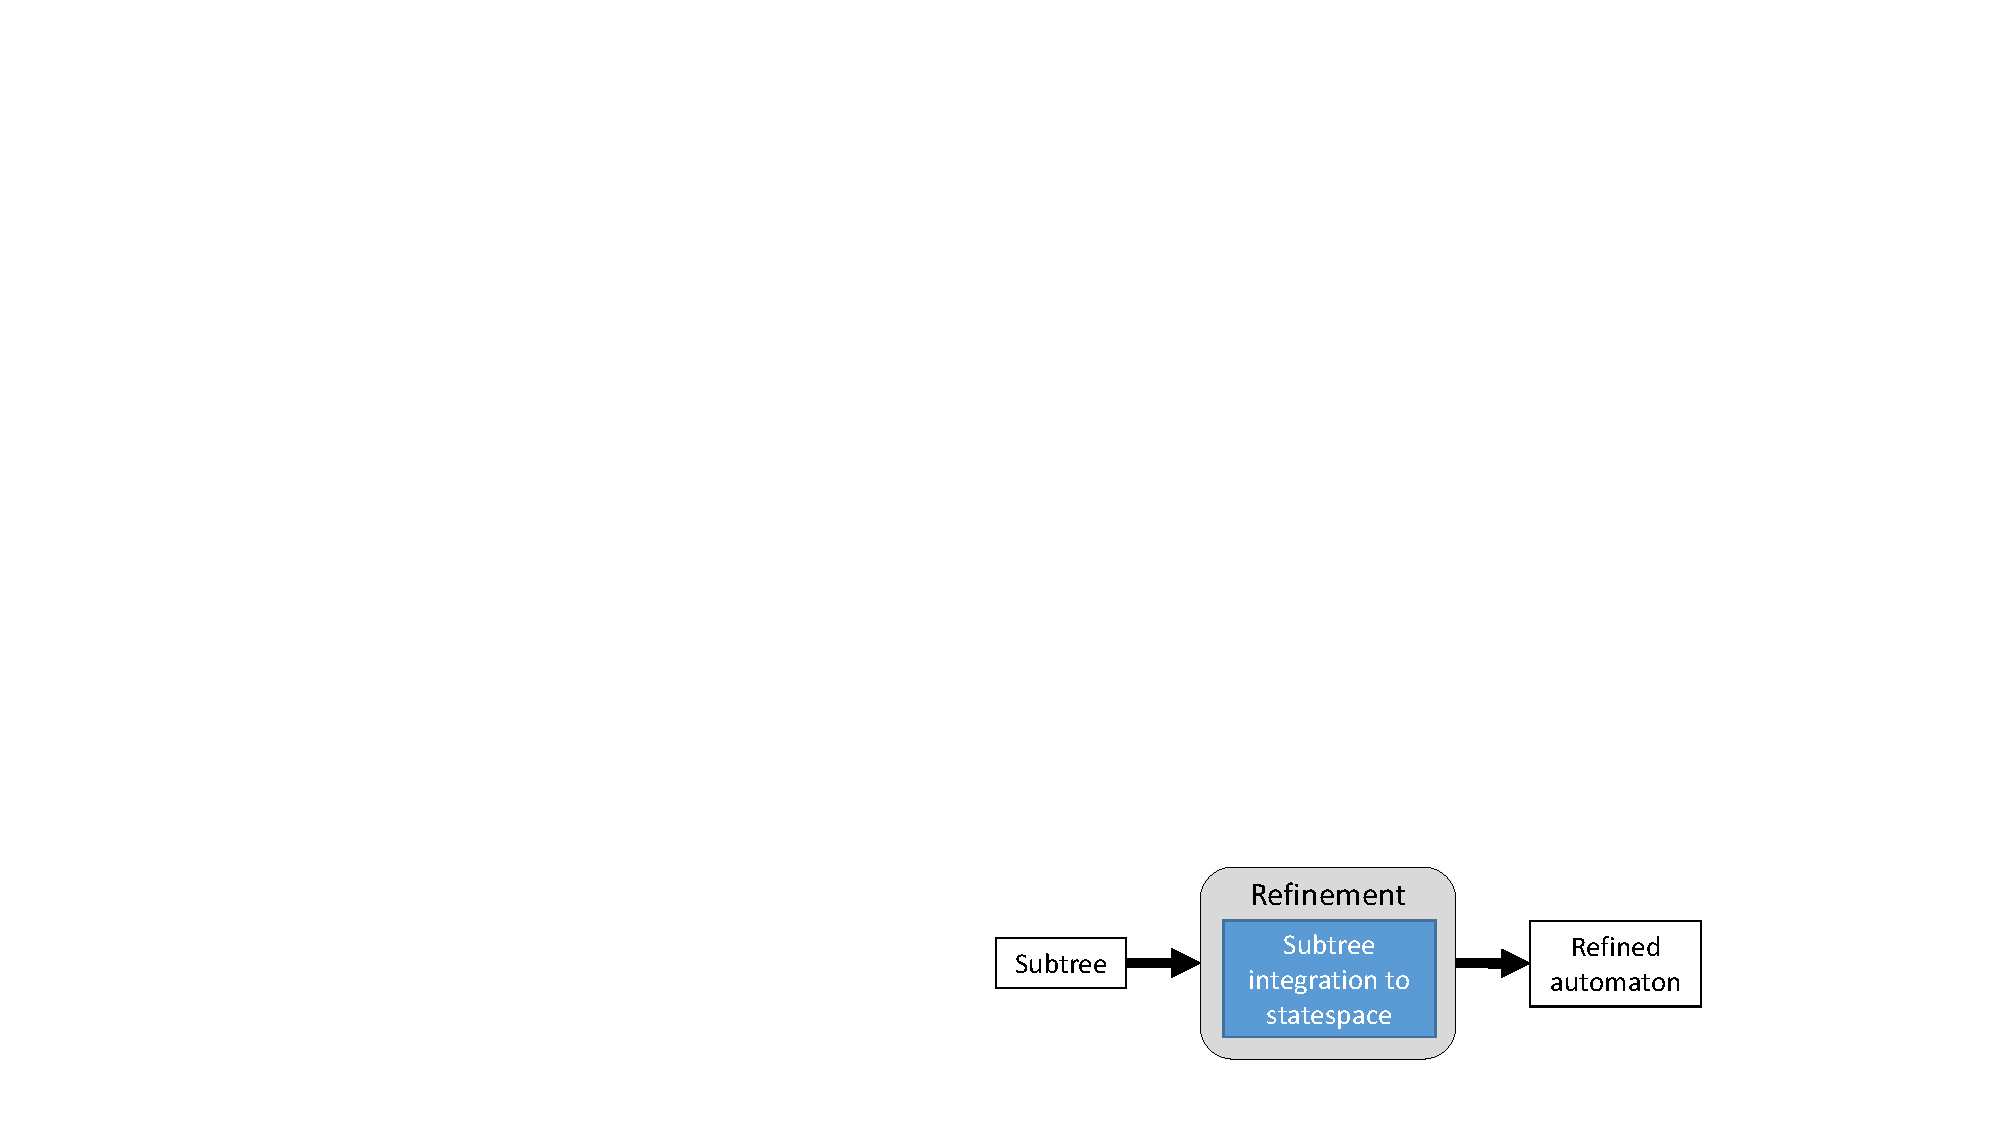
\includegraphics[width=.7\textwidth]{include/figures/modules_ssp_ref}
	%\caption{Statespace-based refinement}
	%\label{fig:cegarssp}
\end{figure}


The next important question is how to integrate the refined tree to the graph. The answer depends on which representation is used.

In case of the graph representation integrating has to be done carefully. Before changing the abstract zone to the refined one we must consider the other incoming edges of the node. The states reachable from that edge may not be contained in the refined zone, and thus if there is an an edge pointing to the node to refine other than the one in the trace, the node should be duplicated, and the other incoming edges should be pointing to the new node (that doesn't get refined). Also, if the result of \emph{split()} is multiple zones, the node has to be replicated, but this time no edges has to be redirected, and one of the refined zones can be assigned to each nodes.

Discrete valuation also has to be calculated at this point. The same discrete valuation has to be assigned for each replicas of the node.

The next step is checking containment. Suppose at one point of the
algorithm the zone $z_{C}$ in node $n$ %of the node $\langle l,z_{C}\rangle$
 is 
refined to  $z_{C'}$ which is a
subzone of a zone $z'_{C'}$ in a node $n'$ containing the same location. In this case any state that is reachable from $n$ is also reachable from $n'$, thus any edge leading to  $n$ can be redirected to $n'$, and $n$ can be removed.

If the erroneous location is reachable through this path, the procedure finds it,
and the CEGAR algorithm terminates. Otherwise, at some point a guard or a target invariant
is not satisfied -- the transition is not enabled. The corresponding edge is removed and the analysis of the path terminates.

\begin{runningExample}
	Integration of the refined trace to the abstraction of the zone graph starts from the first node. Since the zone is still $z_\emptyset$, there is not much to be done. The next node on the trace is $\langle \text{\emph{loop}}, z_\emptyset \rangle$. The loop edge is an incoming edge to the node itself. Thus, the node is duplicated and the loop-edge from the original one is redirected to the new one. Now the zone in the original node can be refined to $x=y \leq 10$. Since \emph{loop} $\to$ \emph{end} is not enabled on the trace, the outgoing edge from $\langle \text{\emph{loop}}, x=y \leq 10 \rangle$ is removed from the graph.
	
	The graph after the process looks as follows.
	\[\langle \text{\emph{start}}, z_\emptyset \rangle \to \langle \text{\emph{loop}}, x=y \leq 10 \rangle \to \langle \text{\emph{loop}}, z_\emptyset \rangle \to \langle \text{\emph{end}}, z_\emptyset \rangle\]
\end{runningExample}

%\todo{pszeudokód?}

Incoming edges that are not on the trace are also important in case of tree representation, however, because of the tree nature of $T$, the other incoming edges of a node $n$ can only be upwards edges, representing that all states represented by some node $n'$ are also represented by $n$. Obviously, this may not be true, after refining the zone in the node, and because of this the edge $n' \to n$ is removed, and $n'$ is marked as unexplored.

Since $T$ is already a tree, it does not cause problems to attach new subtrees to it (because of \emph{split}), but all new nodes have to be marked as unexplored, since only one outgoing edge (of the automaton) were considered when calculating the new subtree, and there could be more.

Containment can also be checked here, just as in case of the graph representation, but it only matters for the leaves of the tree (since the other nodes are already explored). The other possibility is to mark the leaves unexplored and state space exploration will search for containment.

\begin{runningExample}
	Since there are no upwards edges in the current tree, refinement can be performed by replacing the zone in $n_1$ with the refined one and removing edge $n_1 \to n_3$ resulting in the following graph.
	
	\[ \langle \text{\emph{start}}, z_\emptyset \rangle \to \langle \text{\emph{loop}}, x=y \leq 10 \rangle \to \langle \text{\emph{loop}}, z_\emptyset \rangle\] 
\end{runningExample}

%\todo{pszeudokód?}
   



%The zone graph exploratin described in section \ref{sec:tareach} can be used

%Implementált modulok felsorolva, utalással az előző fejezet algoritmusaira. + példák, pszeudokód


\section{Result}

\begin{figure}[h]
	\centering
	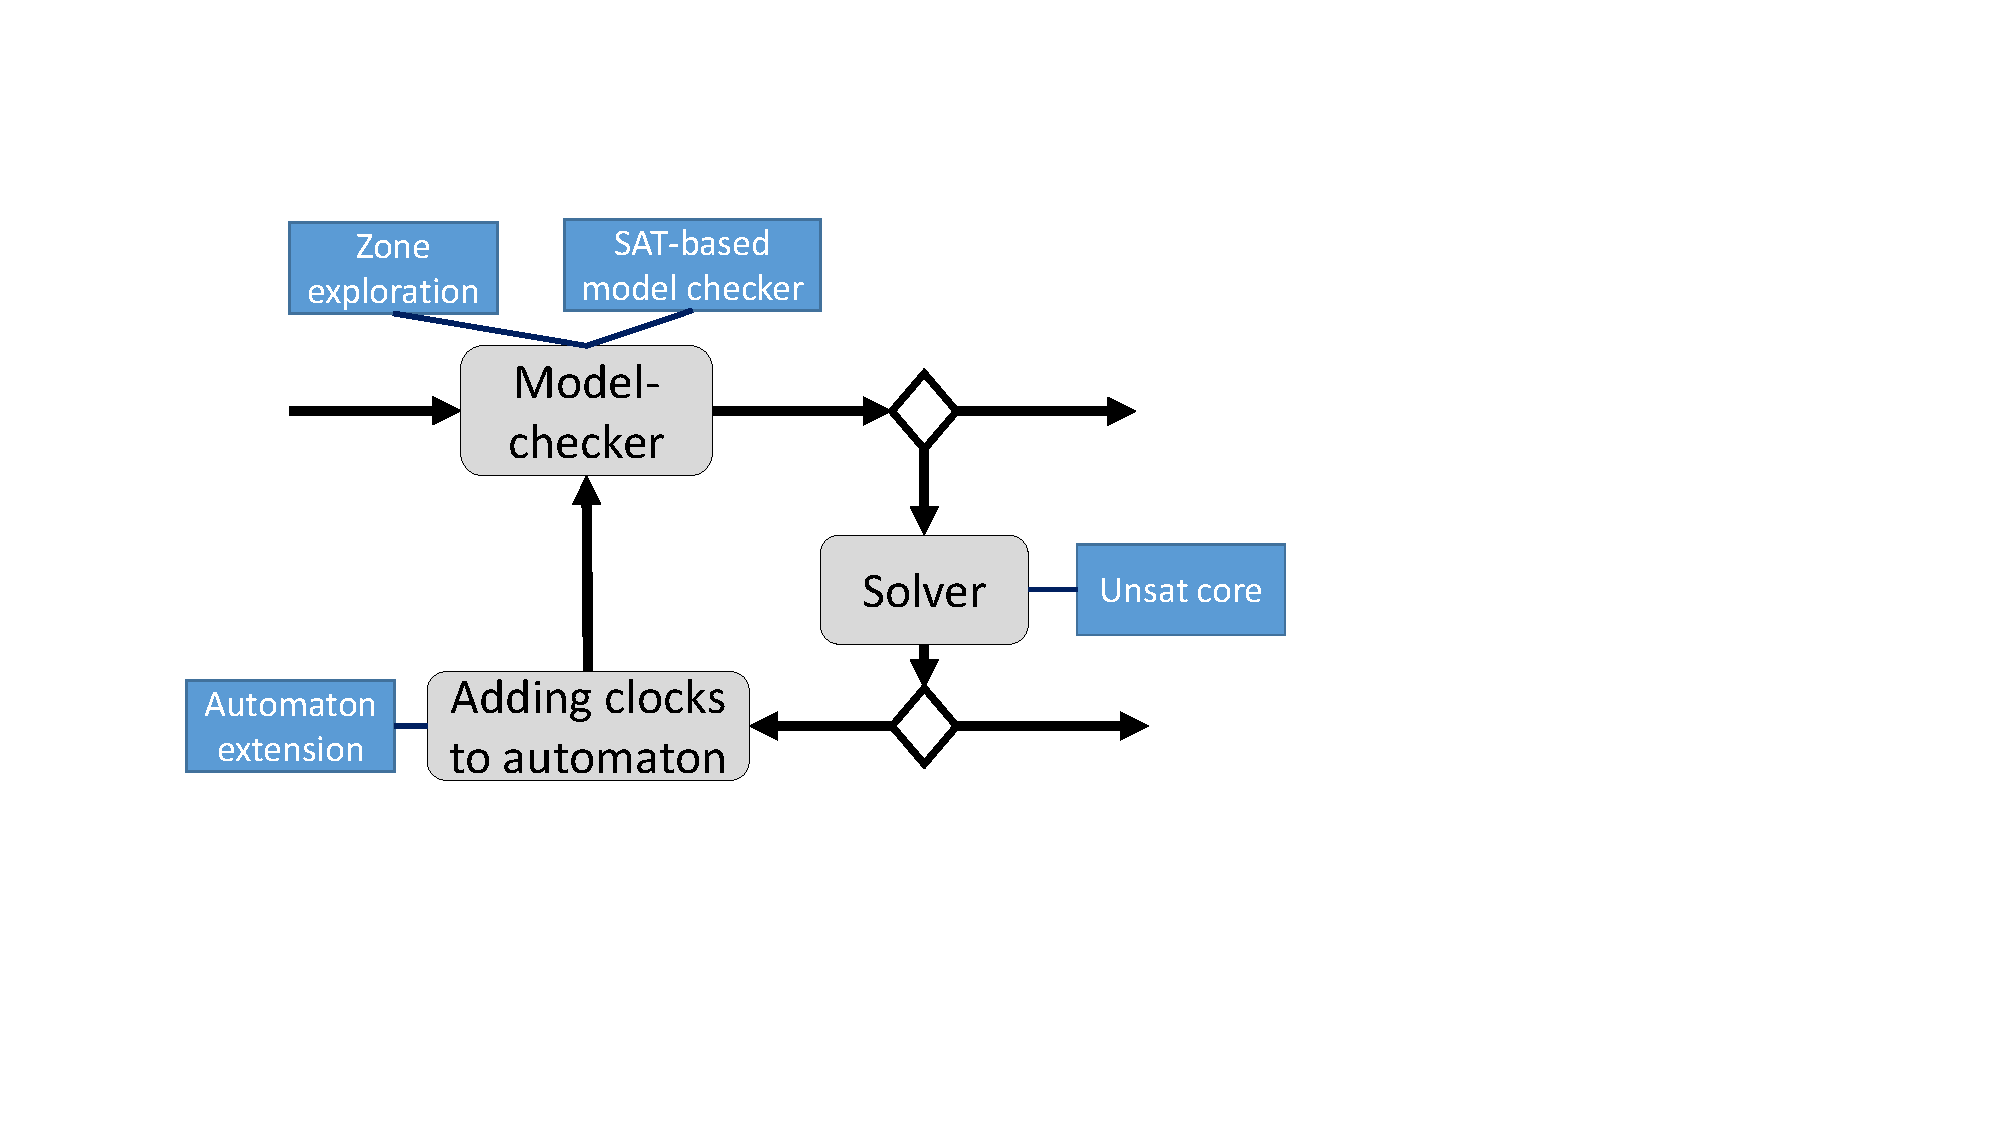
\includegraphics[width=.7\textwidth]{include/figures/cegar_ta_complete}
	\caption{Automaton-based refinement}
	\label{fig:cegartafin}
\end{figure}

Figure \ref{fig:cegartafin} depicts the presented techniques for automaton-based refinement and Figure \ref{fig:cegarsspfin} depicts the presented techniques for state space refinement. In the latter case state space representation-dependent modules are marked with the same colours. Precision and zone calculation are not state space representation-dependent algorithms and can be combined with any of the other colours.

\begin{figure}[h]
	\centering
	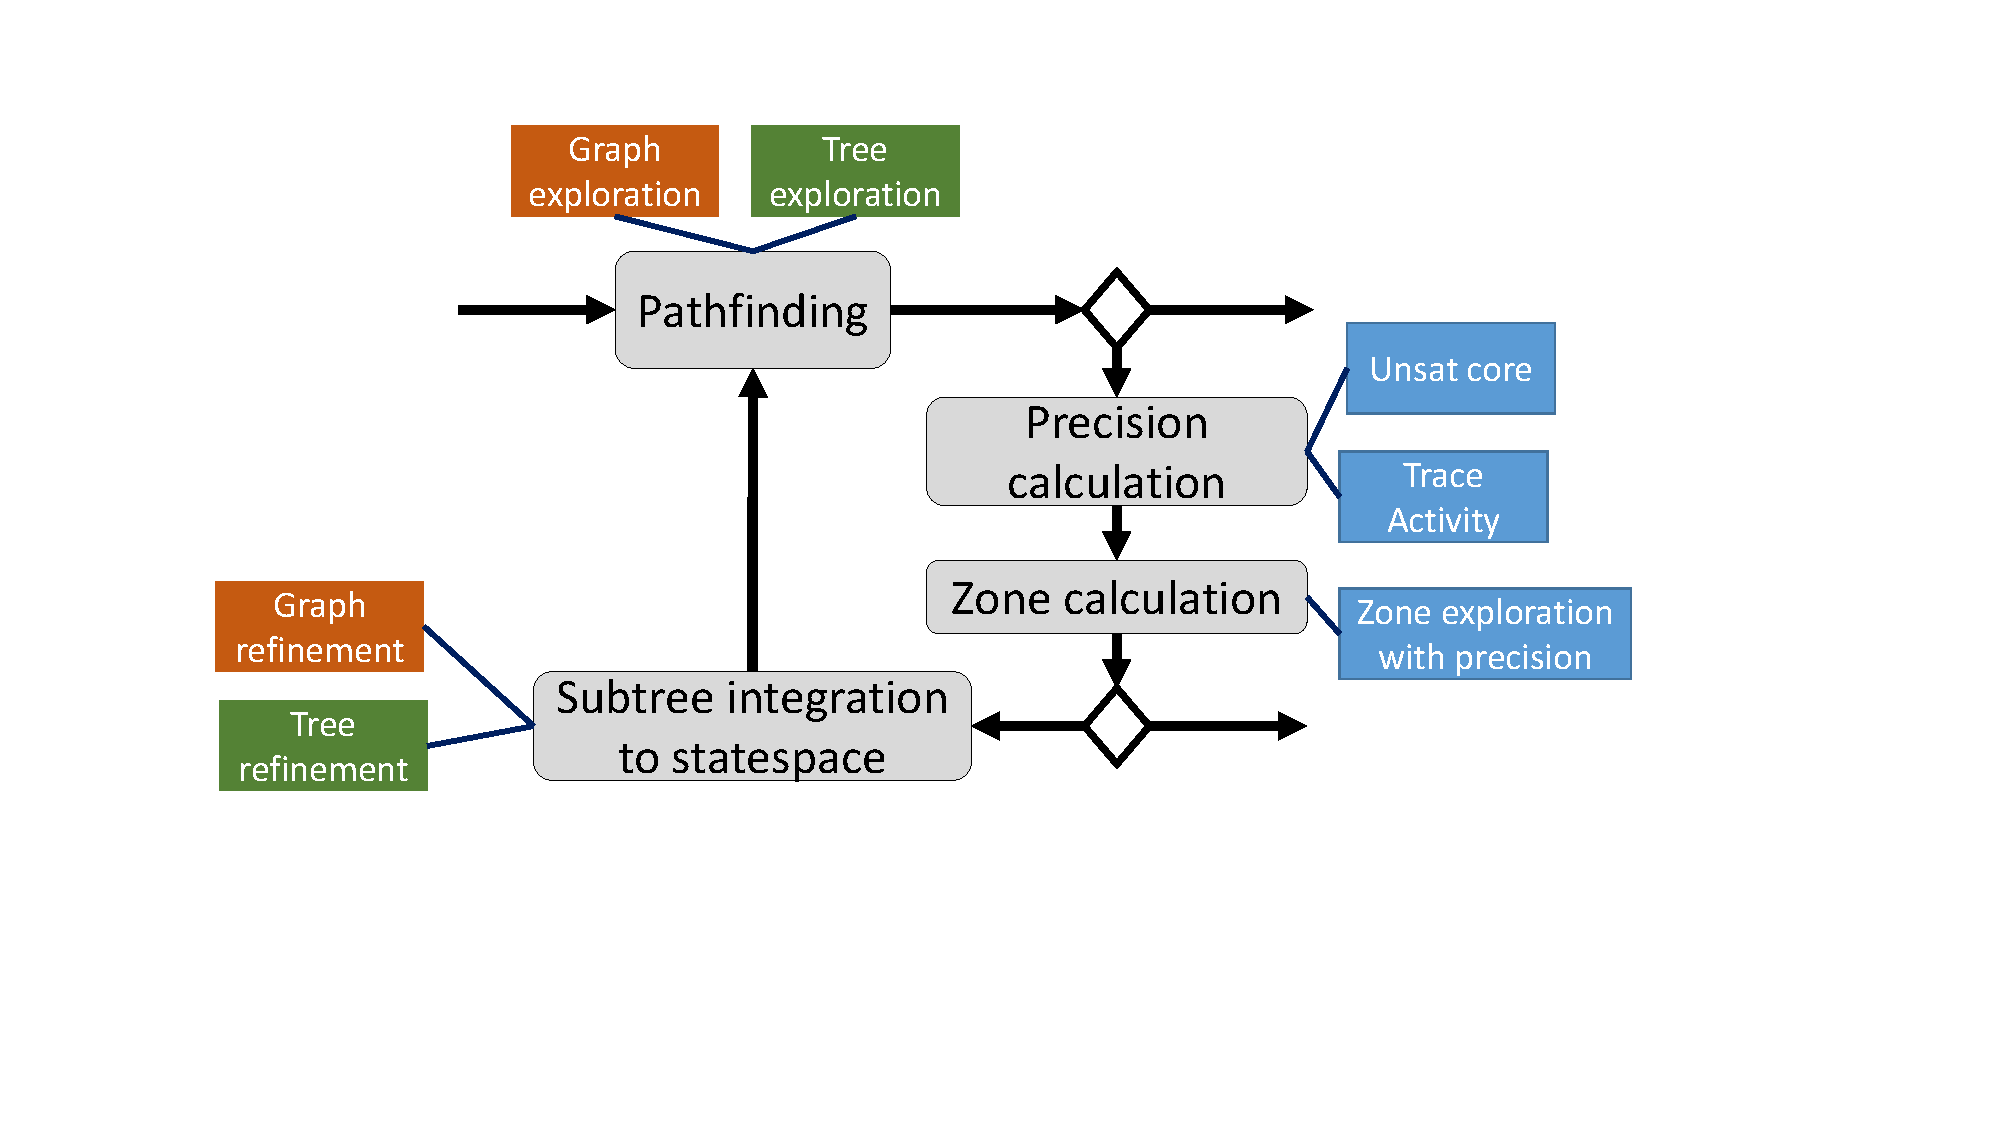
\includegraphics[width=.9\textwidth]{include/figures/cegar_ssp_complete}
	\caption{Statespace-based refinement}
	\label{fig:cegarsspfin}
\end{figure}

The presented framework is extensible in may ways. New techniques can be added to the framework and combined with existing ones, e.g. an online pathfinding algorithm can be studied in place of the current depth first search algorithm represented by the graph exploration module. New representations can be defined for state space-based refinement (e.g. zones can be represented by \emph{potential graphs} \cite{conf/sas/GangeNSSS16}), and even a new aspect of abstraction can be introduced with it's own CEGAR-loop realization (e.g. abstraction can be applied to locations \cite{kemper2007sat}).

A total of six algorithms can be composed of the presented techniques. Two of them apply abstraction to the clock variables of the automaton, similarly to the algorithms presented in papers \cite{dierks2007automatic, he2010compositional,okano2011clock}, while the other four apply abstraction directly to the state space. 


%\todo{Kis szöveg meg sok sok ábra az elkészült algoritmusokról, a kombinálhatóságról, valamint a keretrendszer kiterjesztési lehetőségeiről}
%\subsection{Timed automaton-based refinement with sat based mocdel checker}
%\subsection{Timed automaton-based refinement with sat based mocdel checker}

%
%\todo{Algoritmusok, leírással, hol használják, hogyan lehet TA-ra alkalmazni, miért jó, stb. + hogyan fog beleilleszkedni a konfigurálható izébe (milyen dobozok)}








%\todo{Elkészült dobozok, intefészek, kombinálhatóság}

%\section{}

%\section{Introducing a new algorithm}

%\todo{El kéne nevezni ezt az algoritmust és akkor nem kellene mindenhol "az X. fejezetben bemutatt algoritmus"-ként hivatkozni rá.}

%My algorithm is explained in this section. To ease understanding it is also demonstrated on the automaton in Figure \ref{fig:loopinfinite}, with the error location being the location $end$.

%\subsection{Overview}

 %Due to these disadvantages discussed above I have decided that my approach of applying CEGAR to the reachability analysis of timed automata will modify the reachability algorithm instead of using it as a black box module. My approach applies abstraction to the zone graph of the automaton, instead of the automaton itself. The reachability algorithm (which will now be a CEGAR-based algorithm) will refine the zone graph iteration by iteration until reachability can be decided. The CEGAR loop is interpreted the following way.

 %\begin{description}
 %	\item[Initial abstraction] The key problem about constructing the initial abstraction of the zone graph is that the zone graph is unknown so the abstraction has to be derived from the automaton itself. The idea is really simple: just like the other approaches I also use the location graph of the automaton as the initial abstraction, except in my algorithm it is considered to be the abstraction of the zone graph, not the automaton. To create an overapproximation of the zones, we simply consider every valuations to be reachable in all locations. The zone containing all valuation is denoted by $z_\infty$.
 %	\item[Model checking] Since the abstract zone graph is an abstraction of the reachability graph, model checking becomes a pathfinding problem in the current abstraction of the zone graph. The error location is either proven unreachable or a new trace (path in the graph) is found from the initial node to the target node.
 %	\item[Analysis] This part is about finding out if the error location is really reachable on the trace found in the model-checking phase. The way to do that is by finding out how this path of the abstract zone graph would look like in the refined (real) zone graph. This can be achieved by using the reachability algorithm, but only for the given trace. As discussed in Section \ref{sec:reach}, because of the operation \emph{split} sometimes the real zone graph can branch, which means that the result of the simulation may be a tree instead of a simple path. Nevertheless, it is still easy to decide whether the counterexample is valid: if the error location could be reached by the path (on any branch), then the counterexample is valid. Otherwise, simulation will stop somewhere, typically because one of the transitions (on each branch) is not enabled. In this case the counterexample is spurious.
 %	\item[Refinement] In order to avoid the discussed disadvantages, this algorithm stores as many information of the analysis phase as it can - by replacing the counterexample trace in the abstraction of the zone graph with the calculated subgraph (tree) -- thus refining the abstraction.
 %\end{description}

 
 %\begin{figure} [h]
 %	\centering
 %	\begin{minipage} {0.2\linewidth}%
% 		\vspace*{10pt}%
% 		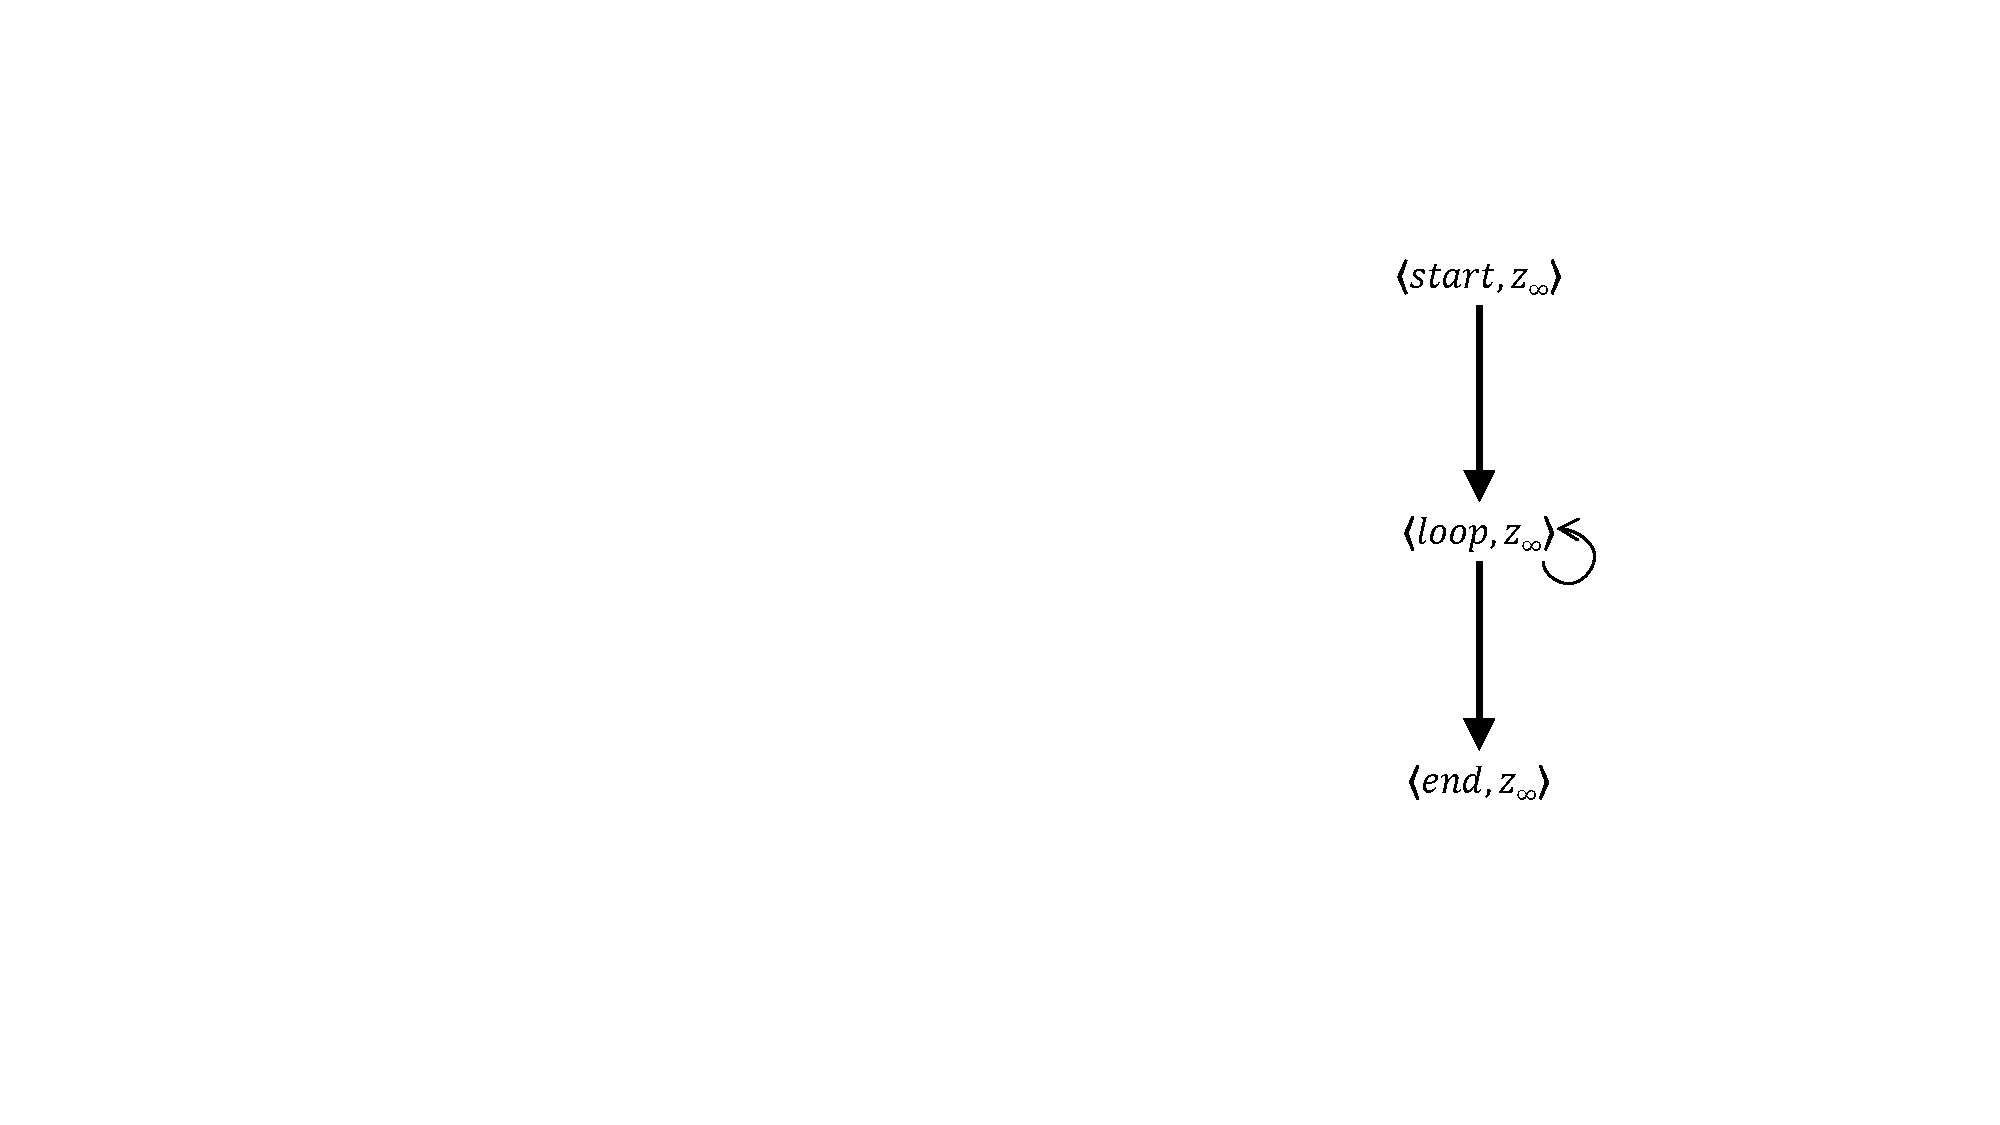
\includegraphics [width=\textwidth]{include/figures/loop_initial_abst}%
% 		\caption{Initial abstraction}
% 		\label{fig:x}
% 	\end{minipage}%
% 	\hspace{20pt}	%
% 	\begin{minipage} {0.2\linewidth}%
% 		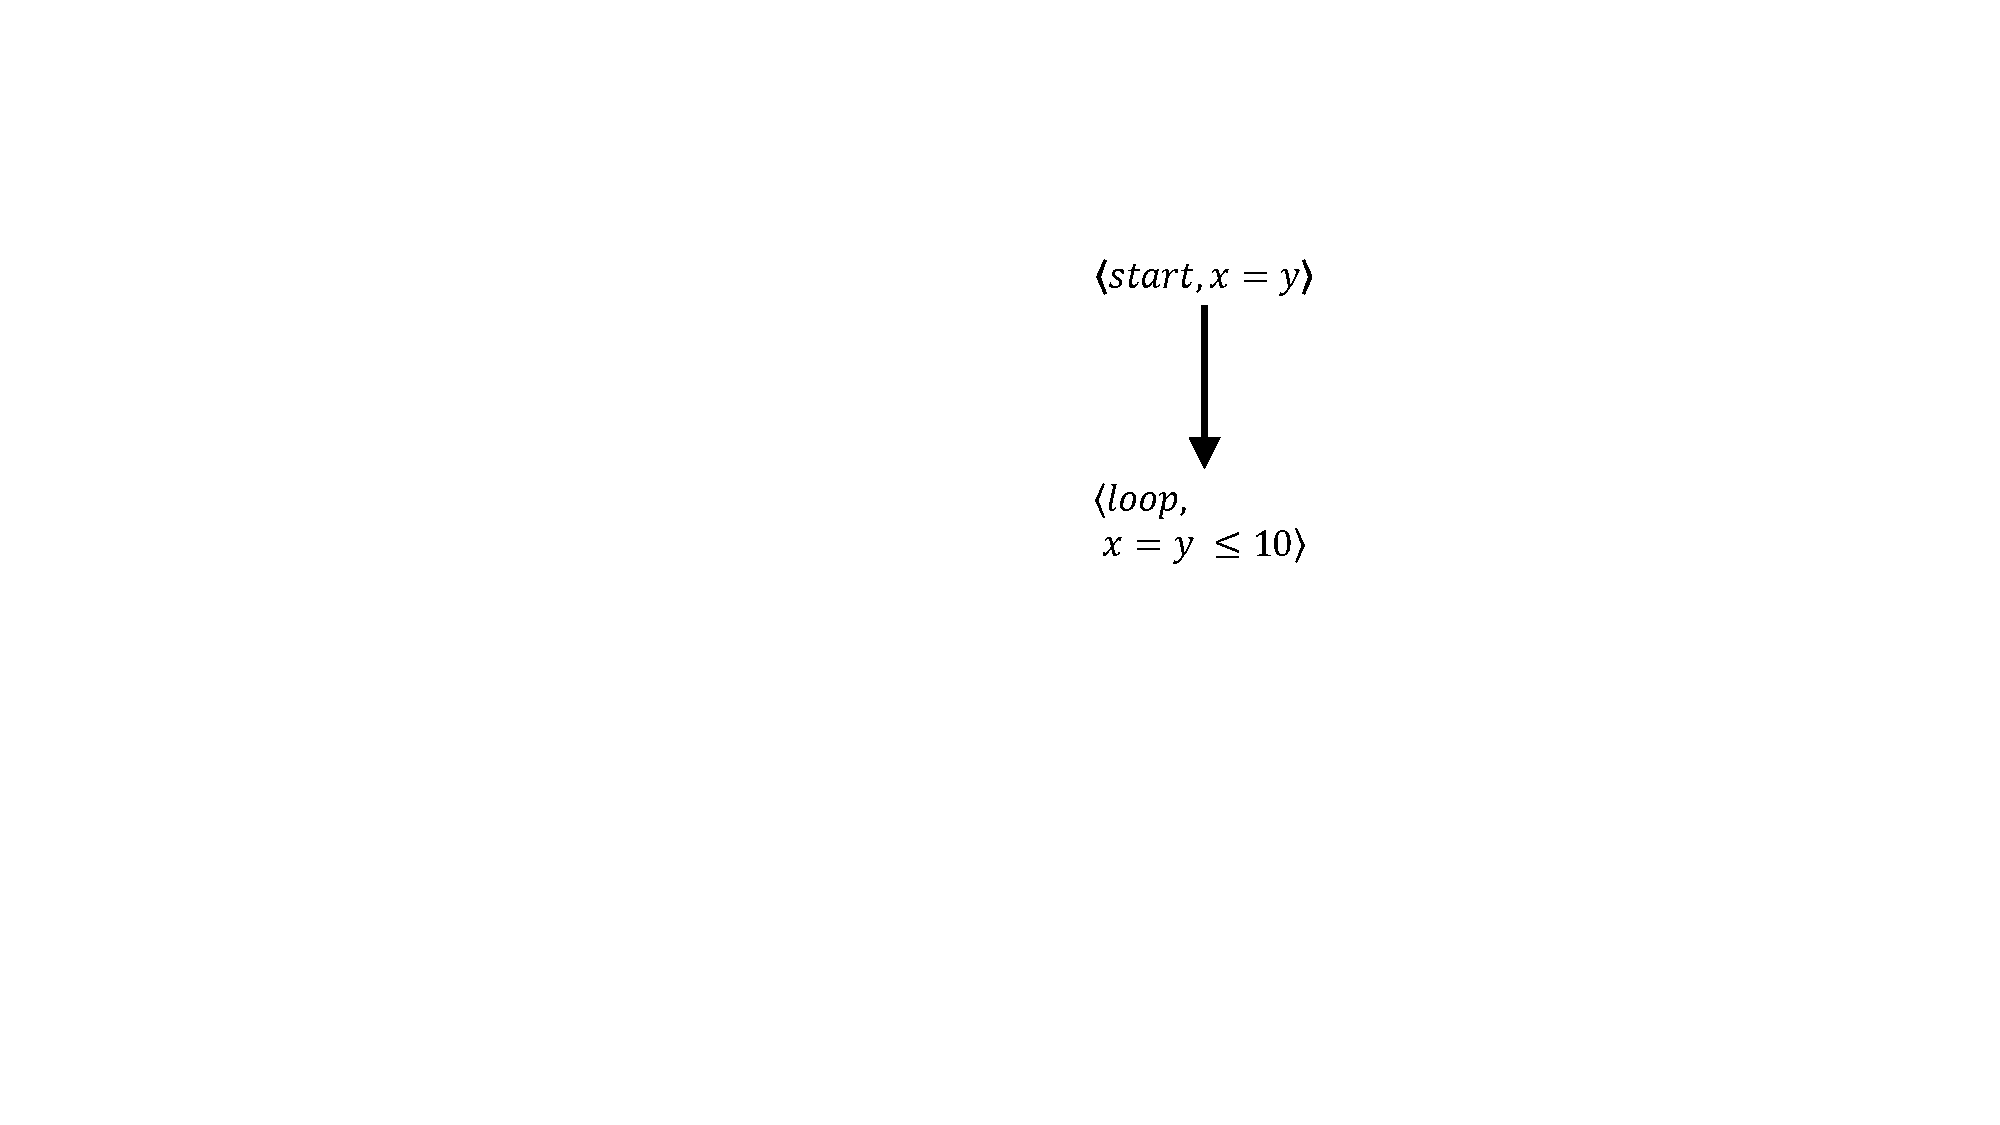
\includegraphics [width=\textwidth] {include/figures/loop_first_ref}%
% 		\vspace*{103pt}%
% 		\caption{Result of analysis}
% 		\label{fig:loopanal}
% 	\end{minipage}%
% 	\hspace{20pt}%
% 	\begin{minipage} {0.25\linewidth}%
% 		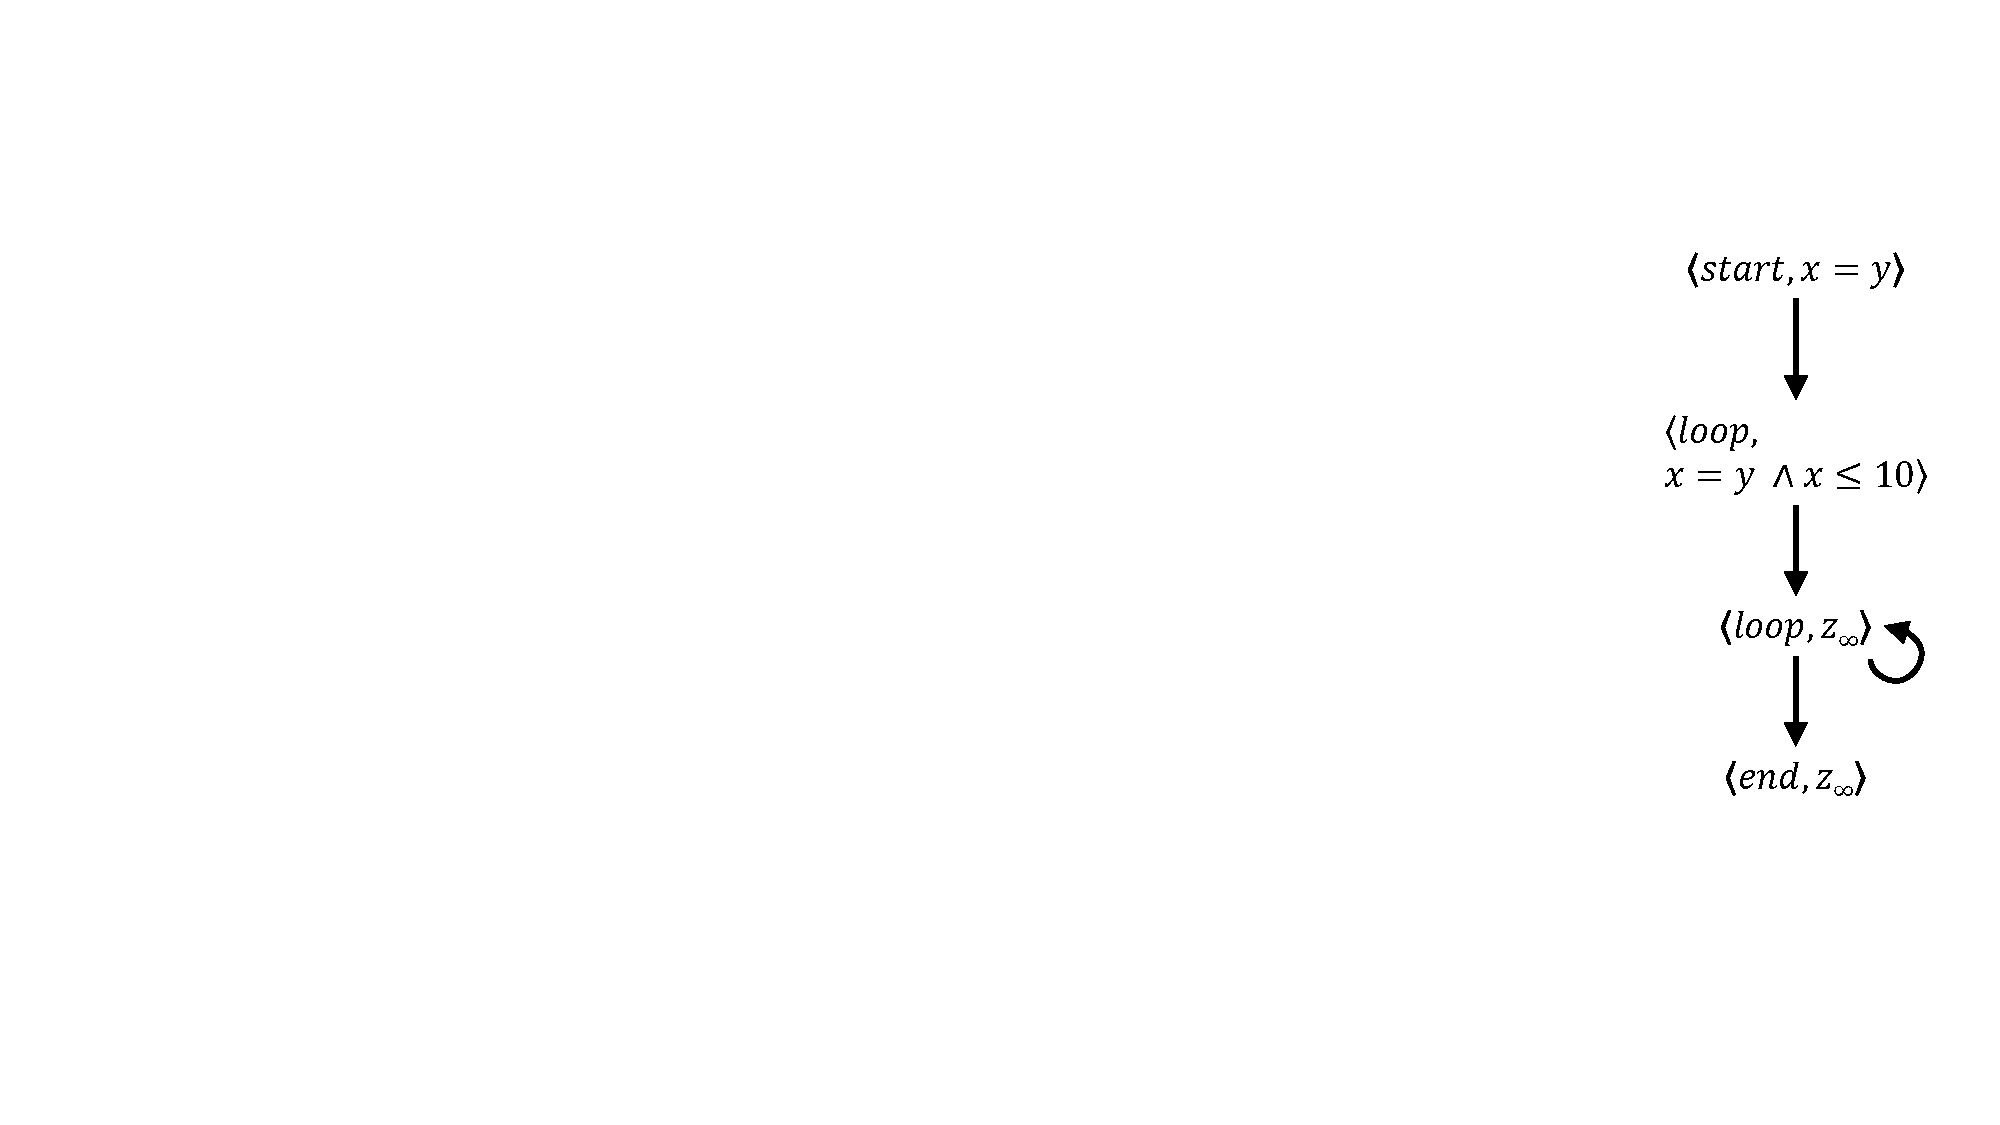
\includegraphics [width=\textwidth] {include/figures/loop_first_abst}%
% 		\vspace*{5pt}%
% 		\caption{After refinement}
% 		\label{fig:loopref}
% 	\end{minipage}
% 	\caption{Timed CEGAR on an example}
% \end{figure}
% 
 
%\subsection{Details}
%
%It is very important to perform the presented operations correctly. This section explains the algorithm step by step, demonstrating it on the example automaton in Figure \ref{fig:loopinfinite}.
%
%Constructing the initial abstraction is very straightforward: each node of the location graph are to be completed with the zone $z_\infty$. After that, model checking is simply a pathfinding in the current abstraction of the zone graph.
%
%\begin{example}
%	The initial abstraction of the example automaton's zone graph is depicted in Figure \ref{fig:x}. The first counterexample is denoted with bold arrows.
%\end{example}
%
%Simulation of the counterexample is performed by constructing the relevant part of the real zone graph. In the first iteration each node on the path will contain $z_\infty$. In this case, refinement starts from the node that belongs to the initial location and the refined zone is calculated as the initial zone of the zone graph.
%
%The result of pathfinding in the graph in Figure \ref{fig:x} is denoted by bold arrows. In case of the later iterations the first few nodes of the
%trace will already be refined, so the refinement can start from the first
%abstract node. The reachable zone should be calculated from the last refined zone,
%considering the guards and the reset as when constructing the zone graph.
%
%When the result of the refinement is more than one zone, the node on the path (and the edge pointing
%to it) is replicated, and one of the refined zones are assigned
%to each resulting node. The refinement can be continued from any of these nodes -- the path branches.
%All of these branches should be analyzed (refined) one by one.
%
%If the erroneous location is reachable through this path, the procedure finds it,
%and the CEGAR algorithm terminates. Otherwise, at some point a guard or a target invariant
%is not satisfied -- the transition is not enabled. The corresponding edge is removed and the analysis of the path terminates.
%
%\begin{example}
%	Consider the example. Since it is the first iteration, we start by constructing the initial node, $\langle start, x=y \rangle$. After that we calculate the next node on the trace $\langle loop, x=y \leq 10 \rangle$. When constructing the zone graph, we continued with the transition represented by the loop-edge but this time we only have to explore the zone graph through the transitions in the counterexample. The next transition is the transition represented by the edge directed to node $\langle end, z_\infty \rangle$. This transition is not enabled in the previously calculated zone, which means the counterexample is spurious. The resulting subgraph of the zone graph is depicted in Figure \ref{fig:loopanal}.
%\end{example}
%
%The goal of refinement is to eliminate the spurious counterexample from the abstract representation. Refinement is applied by replacing the abstract counterexample with the subgraph of the real zone graph calculated in the \emph{Analysis} phase. This operation has to be performed very carefully.
%
%Consider e.g. that the node in the abstract graph that is about to get replaced by one (or more) nodes in the subgraph has other incoming edges than the one in the counterexample. Since it is unknown what states are reachable in the location by the other incoming edges, the node can't be removed. Except, the edge representing the transition in the counterexample has to be redirected to the node with the calculated zone (if there are multiple nodes, it has to be replicated).
%
%Let us suppose that the graph is prepared to place the new node(s). To avoid wasting memory it is advised to use already refined zones in the graph. If the refined zone $z$ of the node $\langle l,z \rangle$ is a subzone of a zone $z'$ in a node $\langle l,z' \rangle$ (both nodes
%contain the same location $l$), then any state that is reachable from $\langle l,z \rangle$ is also reachable from $\langle l,z' \rangle$, thus there is no need to add  $\langle l,z \rangle$ to the graph. Instead, any edge leading to  $\langle l,z \rangle$ should be redirected to $\langle l,z' \rangle$. After that the replacement of the path can not continue from that $\langle l,z' \rangle$, since there might be more states reachable from $\langle l,z' \rangle$ than from $\langle l,z \rangle$. The remaining of the refined zones have to be recalculated and then the replacement can continue.
%
%When replacing the node, the outgoing edges should also be considered. The calculated subtree of the real zone graph only contained the edges in the trace, but in the abstract zone graph there are other outgoing edges of the node. These edges are the outgoing edges of the original (abstract) node in the zone graph, and they have to be replicated, as outgoing edges from the added node(s). After this we can continue with the next node.
%
%\begin{example}
%In the example replacing the initial node can simply be performed by replacing the zone $z_\infty$ with the zone $x=y$. On the other hand, replacing the node $loop$ has to be performed carefully. Since the loop-edge is an incoming edge of the node and is not part of the counterexample, the node can not be replaced. Instead, the incoming edge on the trace is redirected to the new node (in other words, the one to the original node is removed). Since a new node is added, we have to think about it's outgoing edges that are not on the trace -- in this case the only one is the loop edge. For reasons explained before, the loop edge has to be redirected to the abstract version of the node. Thus, the refinement is finished, and now the counterexample is eliminated from the abstract zone graph. Th resulting graph is depicted in Figure \ref{fig:loopref}.
%\end{example}
%
%
%%\section{Realization}
%
%%\todo{Megvalósítós részek ide + pszeudokód}
%
%\section{Evaluation}
%
%It is important to prove that the algorithm is correct, and that it terminates. Both proof relies on that of the original algorithm.
%
%The algorithm always terminates, because the abstraction of zone graph gets refined in every iteration. Even at worst case, the algorithm stops when the zone graph is completely refined.
%
%The algorithm is correct, because the original algorithm is correct. If the algorithm finds a counterexample, it is a trace in the original algorithm. Otherwise, if there is a counterexample in the original algorithm, this algorithm finds it at some point.
%
%
%
%%\todo{Terminálódás, komplexitás, stb.}
